%!TEX root = ../thesis.tex
%*******************************************************************************
%****************************** Third Chapter **********************************
%*******************************************************************************
\chapter{Measurement of the Top Quark Pair Production Cross Section}

The measurement of the top quark production cross section requires multiple steps.
First, the events that are to be used in the measurement need to be selected as described in Section \ref{sec:xsec_sel}.
Based on this selection the simulation is compared to data to assure that the simulation gives a good estimation of the actual measurement (see Section \ref{sec:xsec_datamc}).
On that dataset the cross section is then measured using a template based binned $\chi^2$ fit as described in Section \ref{sec:xsec_fit}.
The templates are chosen to maximize the precision of the analysis as described in Section \ref{sec:xsec_templates}.
Then the fitting procedure and the statistics model are described in more detail in Section \ref{sec:xsec_stat}.
Finally the extrapolation from the full to the fiducial cross section is discussed in Section \ref{sec:xsec_extraction}.

In general the cross section can be measured according to Equation \ref{eq:CaC}. Here $N_{top}$ denotes the number of selected events containing a top quark pair, $A$ denotes the acceptance of the selection,
$\varepsilon$ denotes the efficiency of the selection and $\mathcal{L}$ denotes the luminosity.

\begin{equation}
\sttbar = \frac{N_{top}}{A \cdot \varepsilon \cdot \mathcal{L}}
\label{eq:CaC}
\end{equation} 

Since the selected sample does not only contain top quark pair events the amount of background needs to be determined.
This is done here by fitting template predictions for all relevant background processes and \ttbar to the data.

\section{Event Selection}
\label{sec:xsec_sel}

The aim of the selection is to select a dataset that is dominated by \ttbar events.
At the same time it also defines acceptance and with it the visual phase space, which should be as broad as possible.
This can partially be solved by using different cuts in the different lepton decay channels and then relying on the principle
of lepton universality in the extrapolation.

All events need to fullfill the trigger selection described in detail in Section \ref{sec:Triggersel}.

In the dilepton channel events need two isolated and well defined leptons \todo{Link to reconstruction chapter}.
Both leptons also need to be within the coverage of the tracker fullfilling the condition of $|\eta| < 2.4$.
For electrons the gap region of the electronic calorimeter $1.4442<|\eta|<1.566$ is vetoed as well.
The decay is then defined according to the two leptons leading in \pt requiring the leading lepton to have $\pt > 25 \GeV$
and the sub leading lepton to have $\pt > 20 \GeV$. 
According to these two leptons the events are then classified into the \emu,\ee and \mumu channels.

The mass of the dilepton system is required to have $\mll > 20 \GeV$ to avoid contamination from low mass DY events.
In the same-flavor channels the window of the Z-mass resonance is vetoed $76 \GeV < \mll <106 \GeV$ to reduce the dominant background of 
resonant Drell-Yan production.

Jets are required to have $\pt > 30 \GeV$ and $|\eta|<2.4$. In order to identify b-tagged jets a tight working point is chosed, giving as high 
purity for selected b-tagged jets.

In the same flavor channels events are required to contain one b-tagged jets, while in the \emu channel does not include any requirement on the jets.

The visible phase space is defined according to the cuts in the \emu channel as it has the highest acceptance:
The leading lepton is required to have $\pt > 25 \GeV$ and the sub leading lepton is required to have $\pt > 20 \GeV$ with the dilepton system
fullfilling $\mll > 20 \GeV$. The principle of lepton universality allows to assume that the regions of the phase space that are additionally cut in the 
same flavor channels can be covered by assuming the same behaviour as in the \emu channel.
The visible phase space also defines the acceptance which is the correction from the full to the visible phase space.



\subsection{Comparison of Simulation and Data}
\label{sec:xsec_datamc}

\section{Extracting the Cross Section}
\label{sec:xsec_fit}

As given in Equation \ref{eq:CaC} the cross section depends on three variables, $N_{top}$,$\varepsilon$, $A$, while the luminosity is given by a different measurement.
These three variables have to be determined in order to measure the cross section. 

Here, this is done with a binned $\chi^2$ fit where the templates for \ttbar and background events taken from simulation are fitted to data distributions and systematic uncertainties are treated as nuisance parameters.
Including the systematic uncertainties as nuisance parameters allows to reduce their impact on the cross section measurement, depending on the choice of templates and event classification.


The acceptance is defined as the fraction of the visible to the full phase space (see Section \ref{sec:xsec_sel} for the definition of the visible phase space).
Since the measurement can only be done in the visible phase space this value has to be taken from simulation. The acceptance can only be constrained within the visible phase space.

The nominal value for the efficiency is taken from simulation as well.  But here, the simulation has been corrected for the efficiency in data as explained in \todo{Link to SFs}. 
As the efficiency for all selected physics objects has been measured in data the efficiency value from simulation corresponds to the efficiency in data.
Since the efficiency is measured in data it can be fully constrained within the measurement.

The templates for the fit are separated first separated according to the dilepton decay channel. Since the efficiencies for the muon and electron reconstruction are correlated in all the channels and the \emu channel depends on both this separation allows to constrain the higher of the two lepton related uncertainties.

They are further subdivided into categories of the number of b-tagged jets in order to distinguish between \ttbar and background events. There are three subcategories of events with one, two and zero or more than two b-tagged jets.

This allows an explicit and independent determination of the efficiency of the b-tagging algorithm for data and simulation depending on the nuisance parameters. The efficiency of the b-tagging algorithm is the same in all three dilepton decay channels.
Directly measuring the b-tagging efficiency in the phase space of the measurement is also expected to reduce the impact of the uncertainties of the b-tagging efficiency measurement on the final measurement of the \ttbar cross section.


\subsection{The Choice of Sensitive Templates}
\label{sec:xsec_templates}

The choice of templates is an important part of the fitting procedure.
The variables that are used should both allow to further separate signal and background processes and at the same time be sensitive to systematic
variations in order to constrain their impact on the final result.

As the b-tagging efficiency is already determined intrinsically the fit will already be sensitive to the related nuisance parameters.
Beside the number of b-jets the number of light jets is one of the main discriminators between \ttbar and background events.
Together with the \pt of the light jets it is also sensitive to the systematic uncertainty on the response of the jet reconstruction and
the systematic uncertainties introduced by theoretical assumptions in the simulation.
These systematic uncertainties make large contributions to the \ttbar cross section measurement \todo{Link to CC}, so reducing
them should help to improve on previous measurements.

The final templates are shown in Figures \ref{fig:xsec_emu_inputdistr,fig:xsec_mumu_inputdistr,fig:xsec_ee_inputdistr} for the \emu,\mumu and \ee channel respectively. The events are divided first by the dilepton decay channel, then by number of b-tagged jets and 
then by the number of additional light jets resulting in twenty eight distributions overall.

\begin{figure}[htbp!]
  \begin{center}
    \resizebox{0.24 \textwidth}{!}{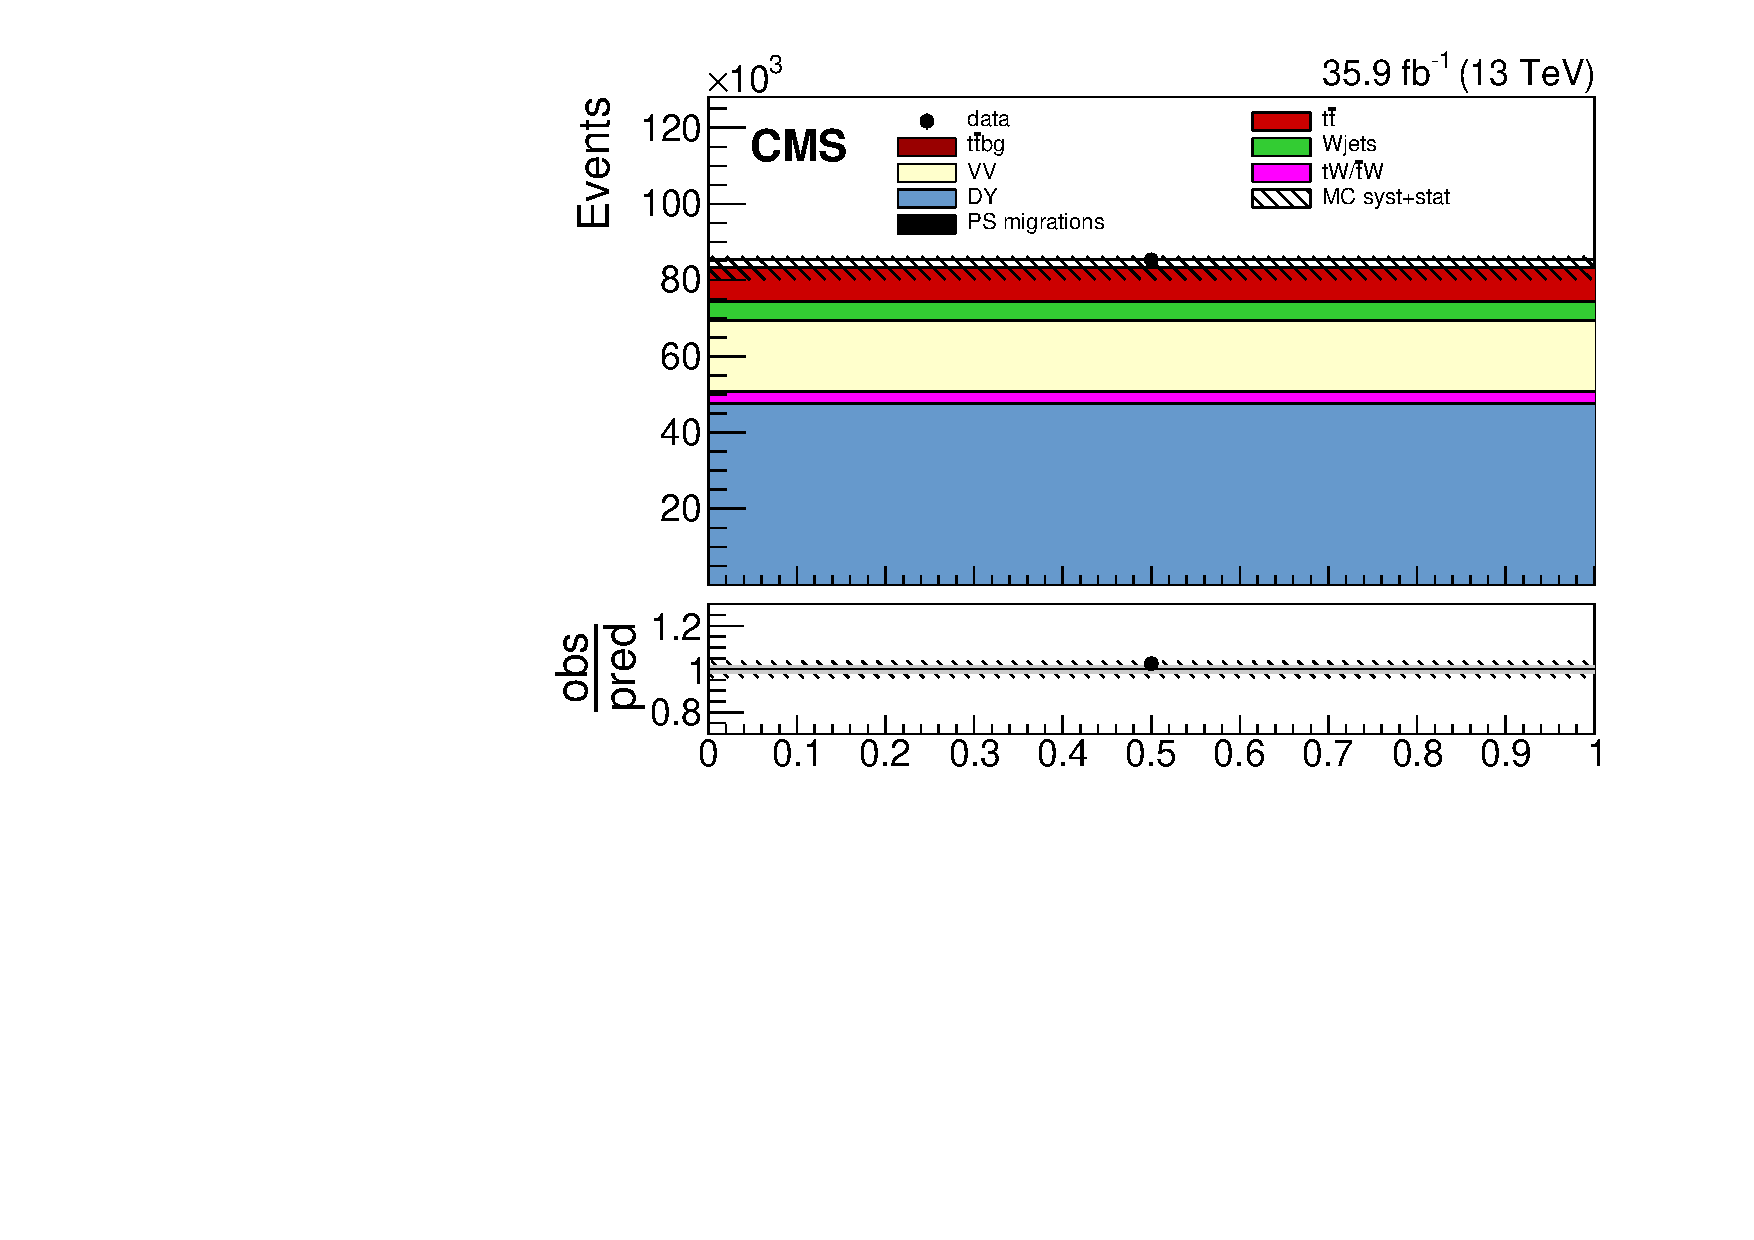
\includegraphics{CrossSection/Figures/ControlPlots/emu_sysnom/total_0_0_b-jets_step_8.pdf}}
    \resizebox{0.24 \textwidth}{!}{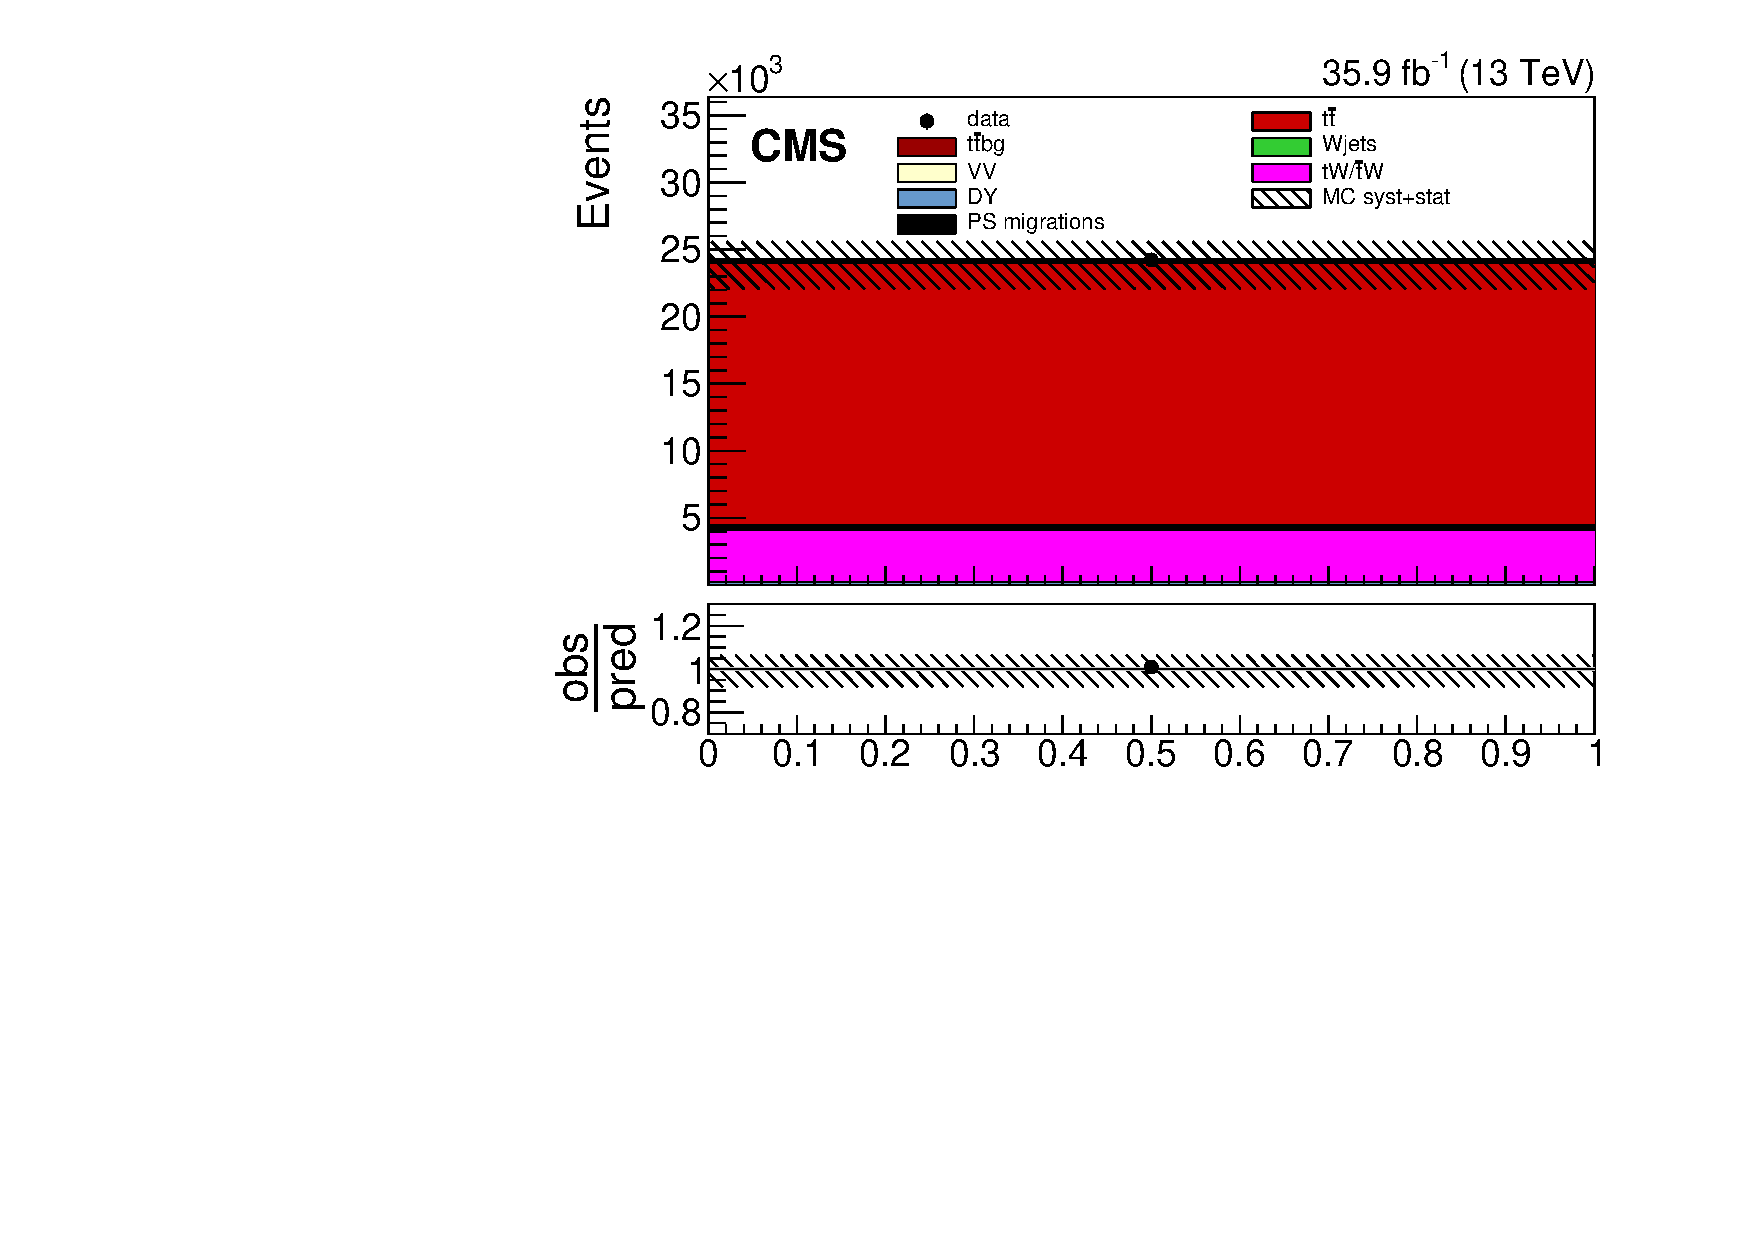
\includegraphics{CrossSection/Figures/ControlPlots/emu_sysnom/total_1_0_b-jets_step_8.pdf}}
    \resizebox{0.24 \textwidth}{!}{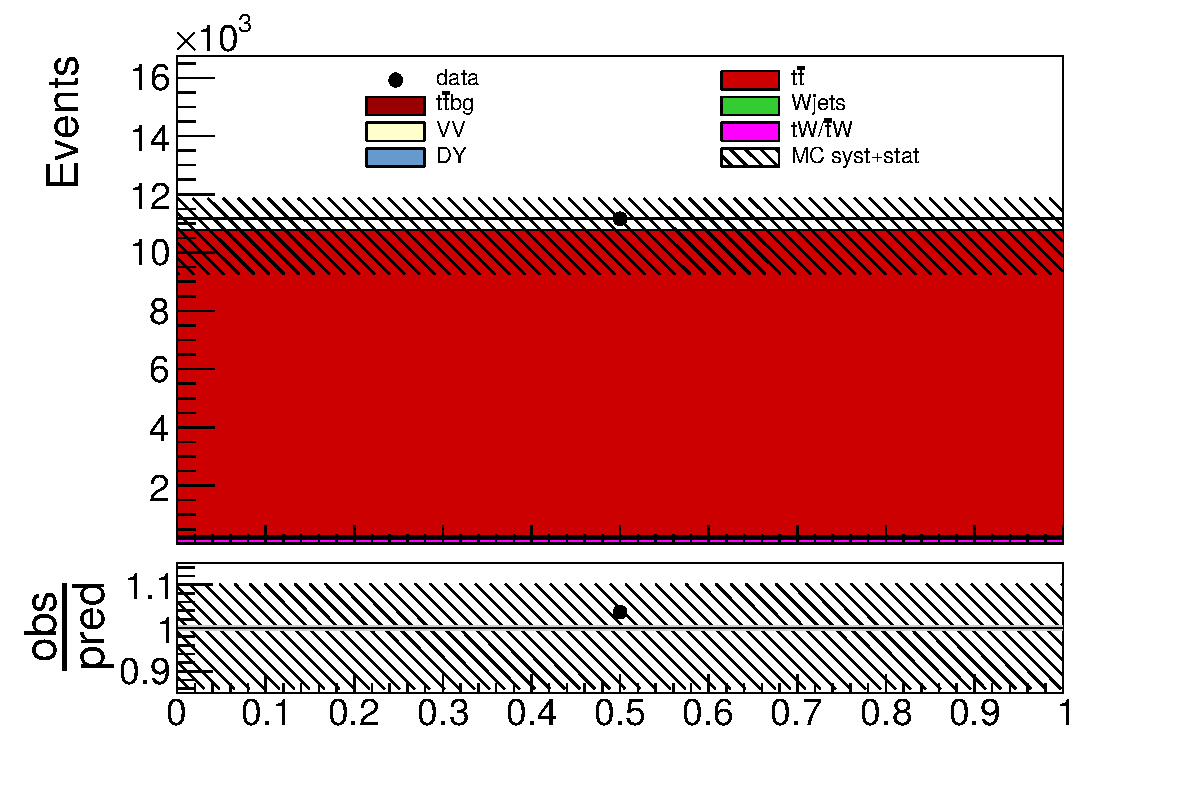
\includegraphics{CrossSection/Figures/ControlPlots/emu_sysnom/total_2_0_b-jets_step_8.pdf}}

    \resizebox{0.32 \textwidth}{!}{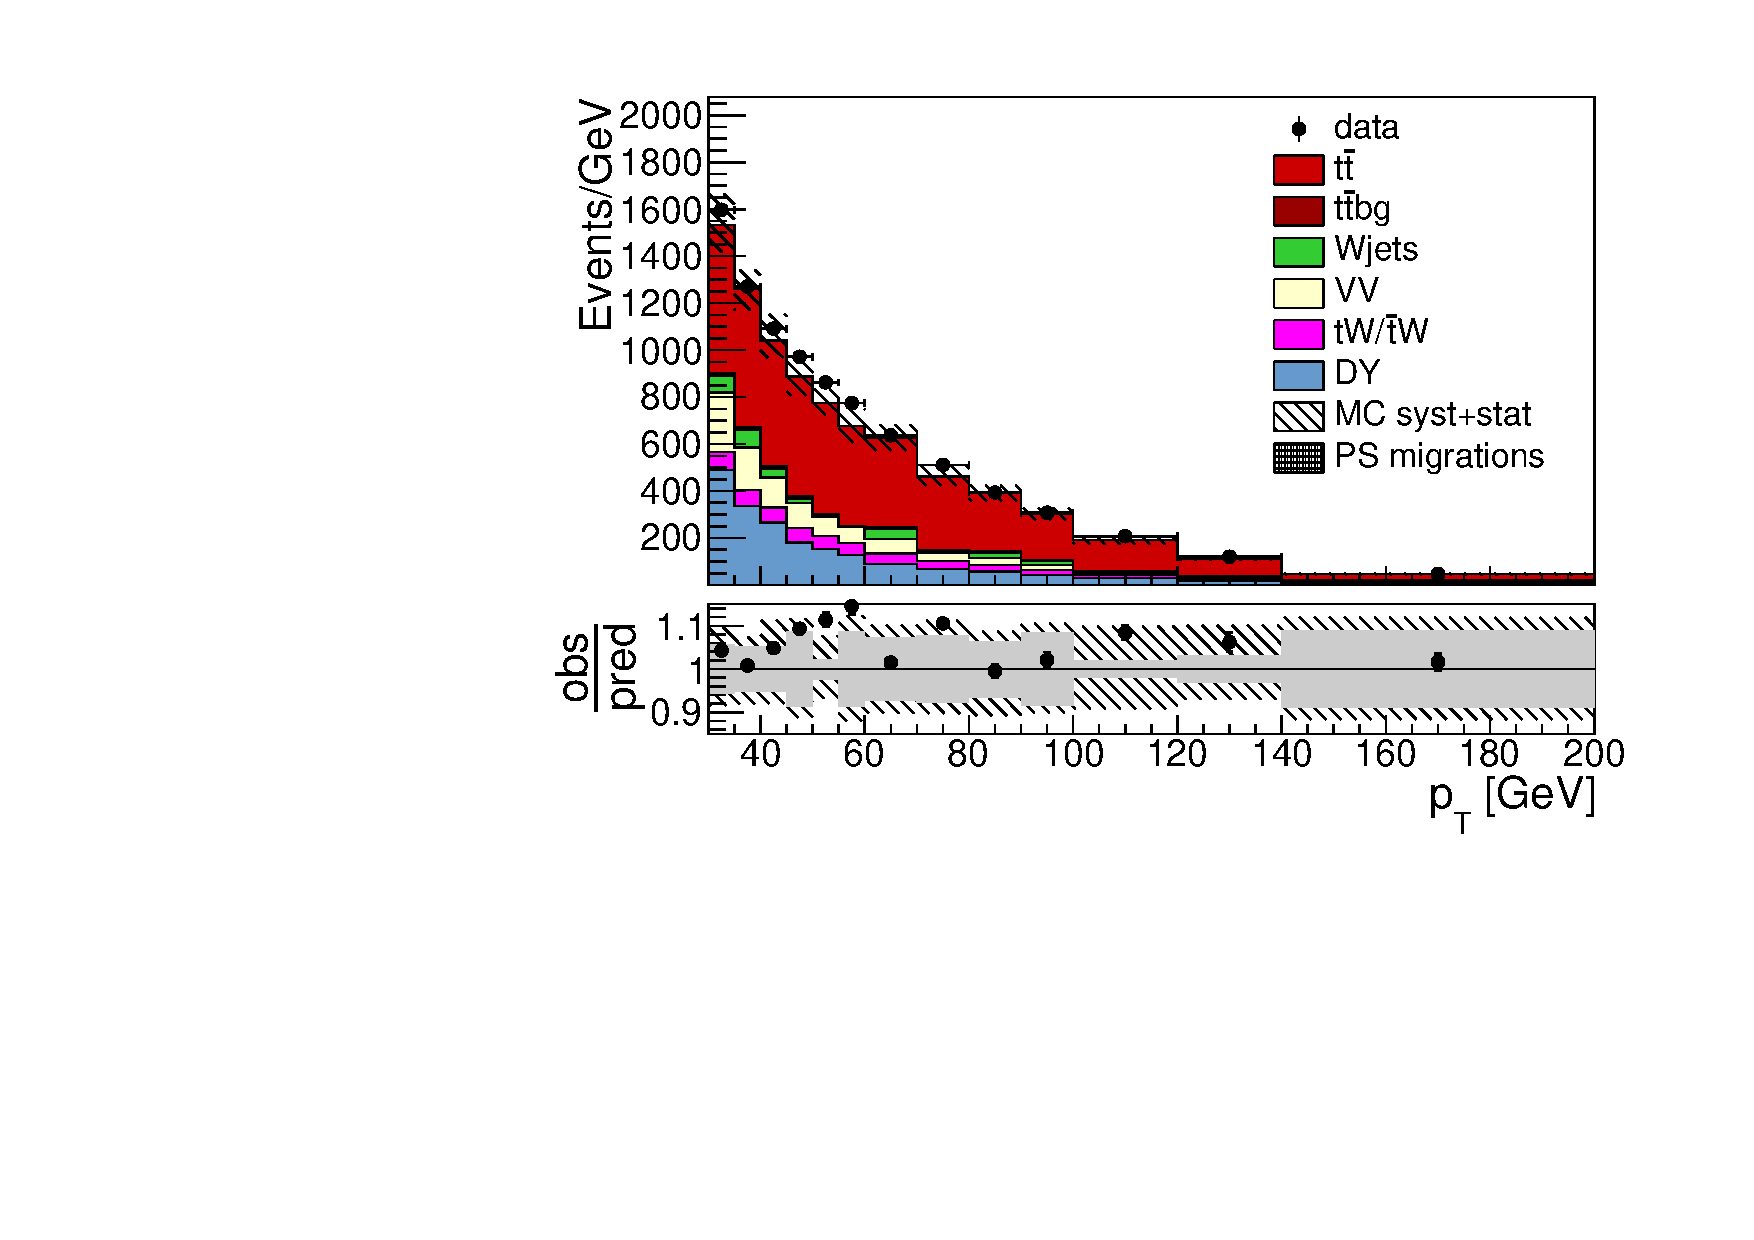
\includegraphics{CrossSection/Figures/ControlPlots/emu_sysnom/lead_jet_pt_0_1_b-jets_step_8.pdf}}
    \resizebox{0.32 \textwidth}{!}{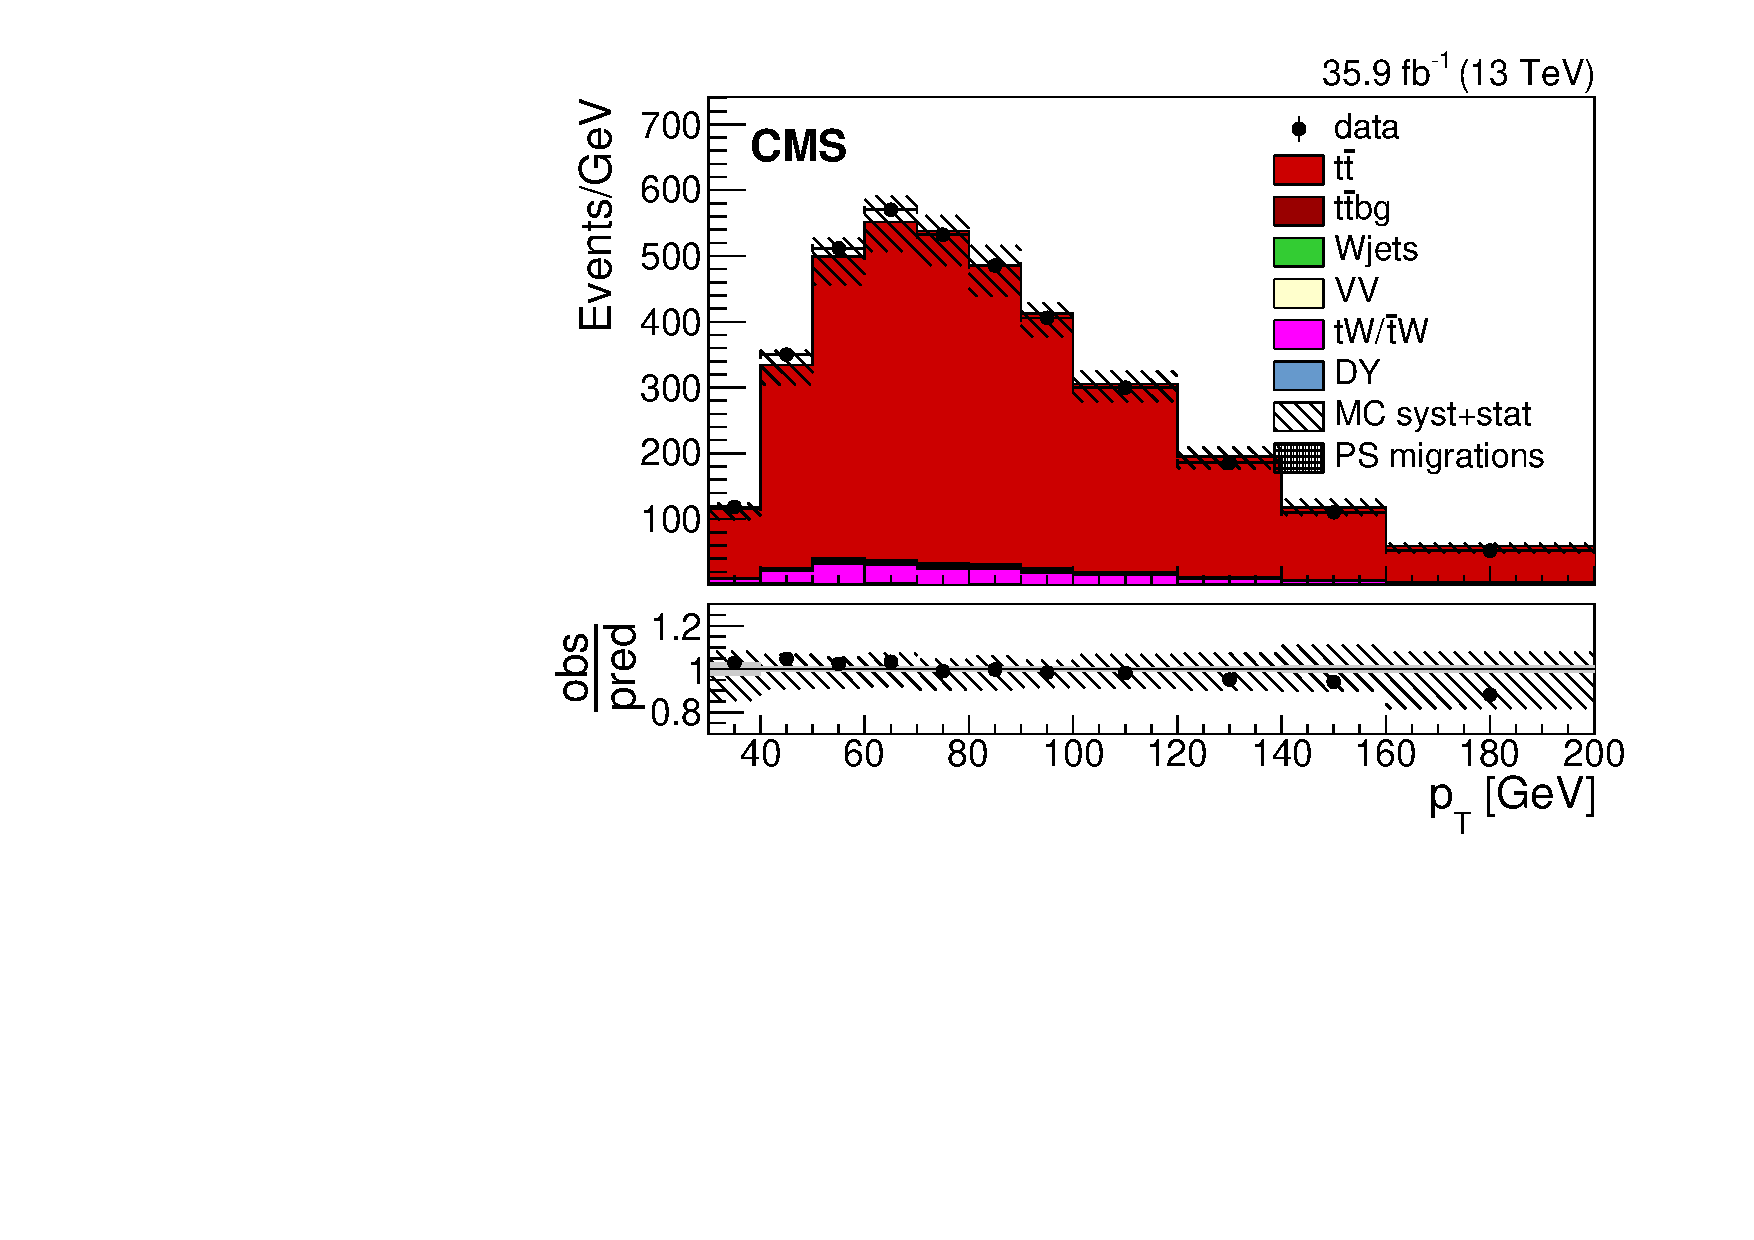
\includegraphics{CrossSection/Figures/ControlPlots/emu_sysnom/lead_jet_pt_1_1_b-jets_step_8.pdf}}
    \resizebox{0.32 \textwidth}{!}{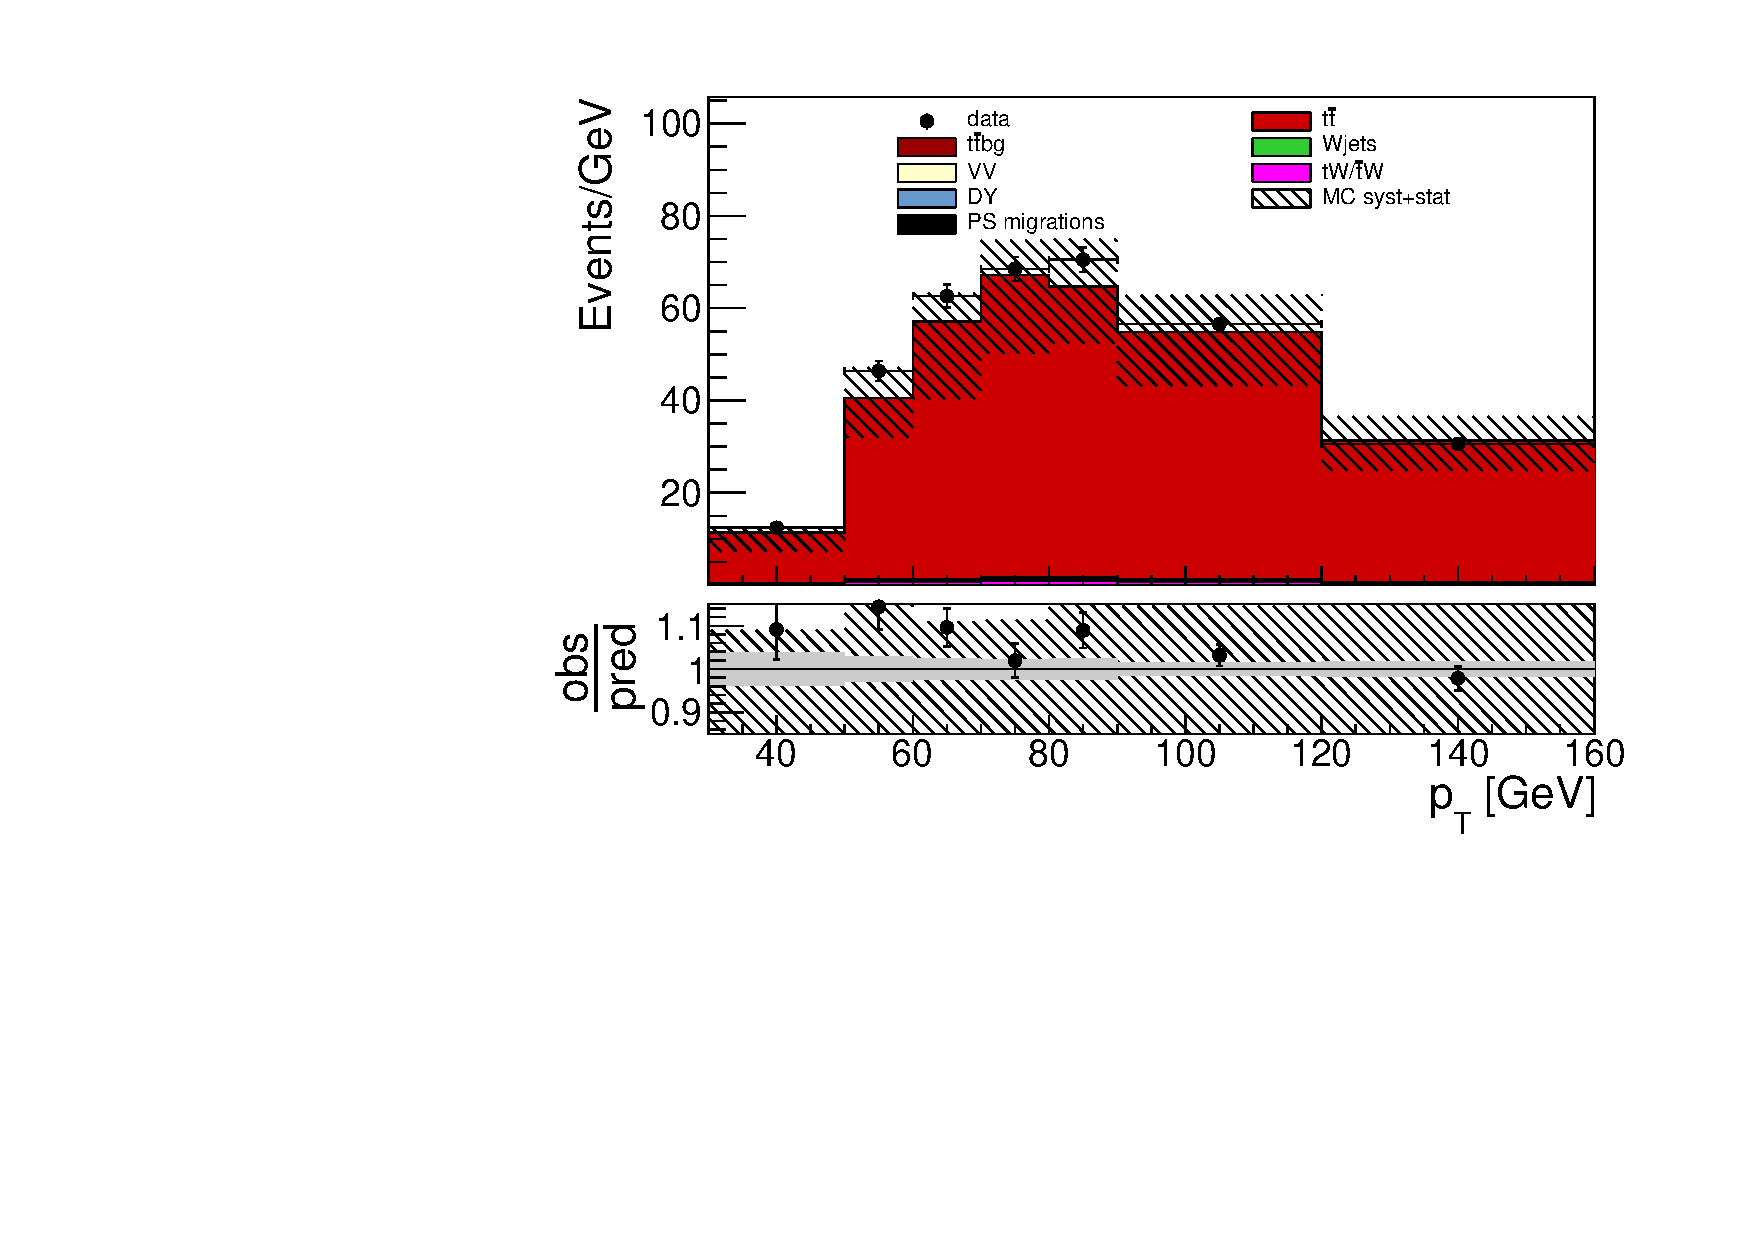
\includegraphics{CrossSection/Figures/ControlPlots/emu_sysnom/lead_jet_pt_2_1_b-jets_step_8.pdf}}
        
    \resizebox{0.32 \textwidth}{!}{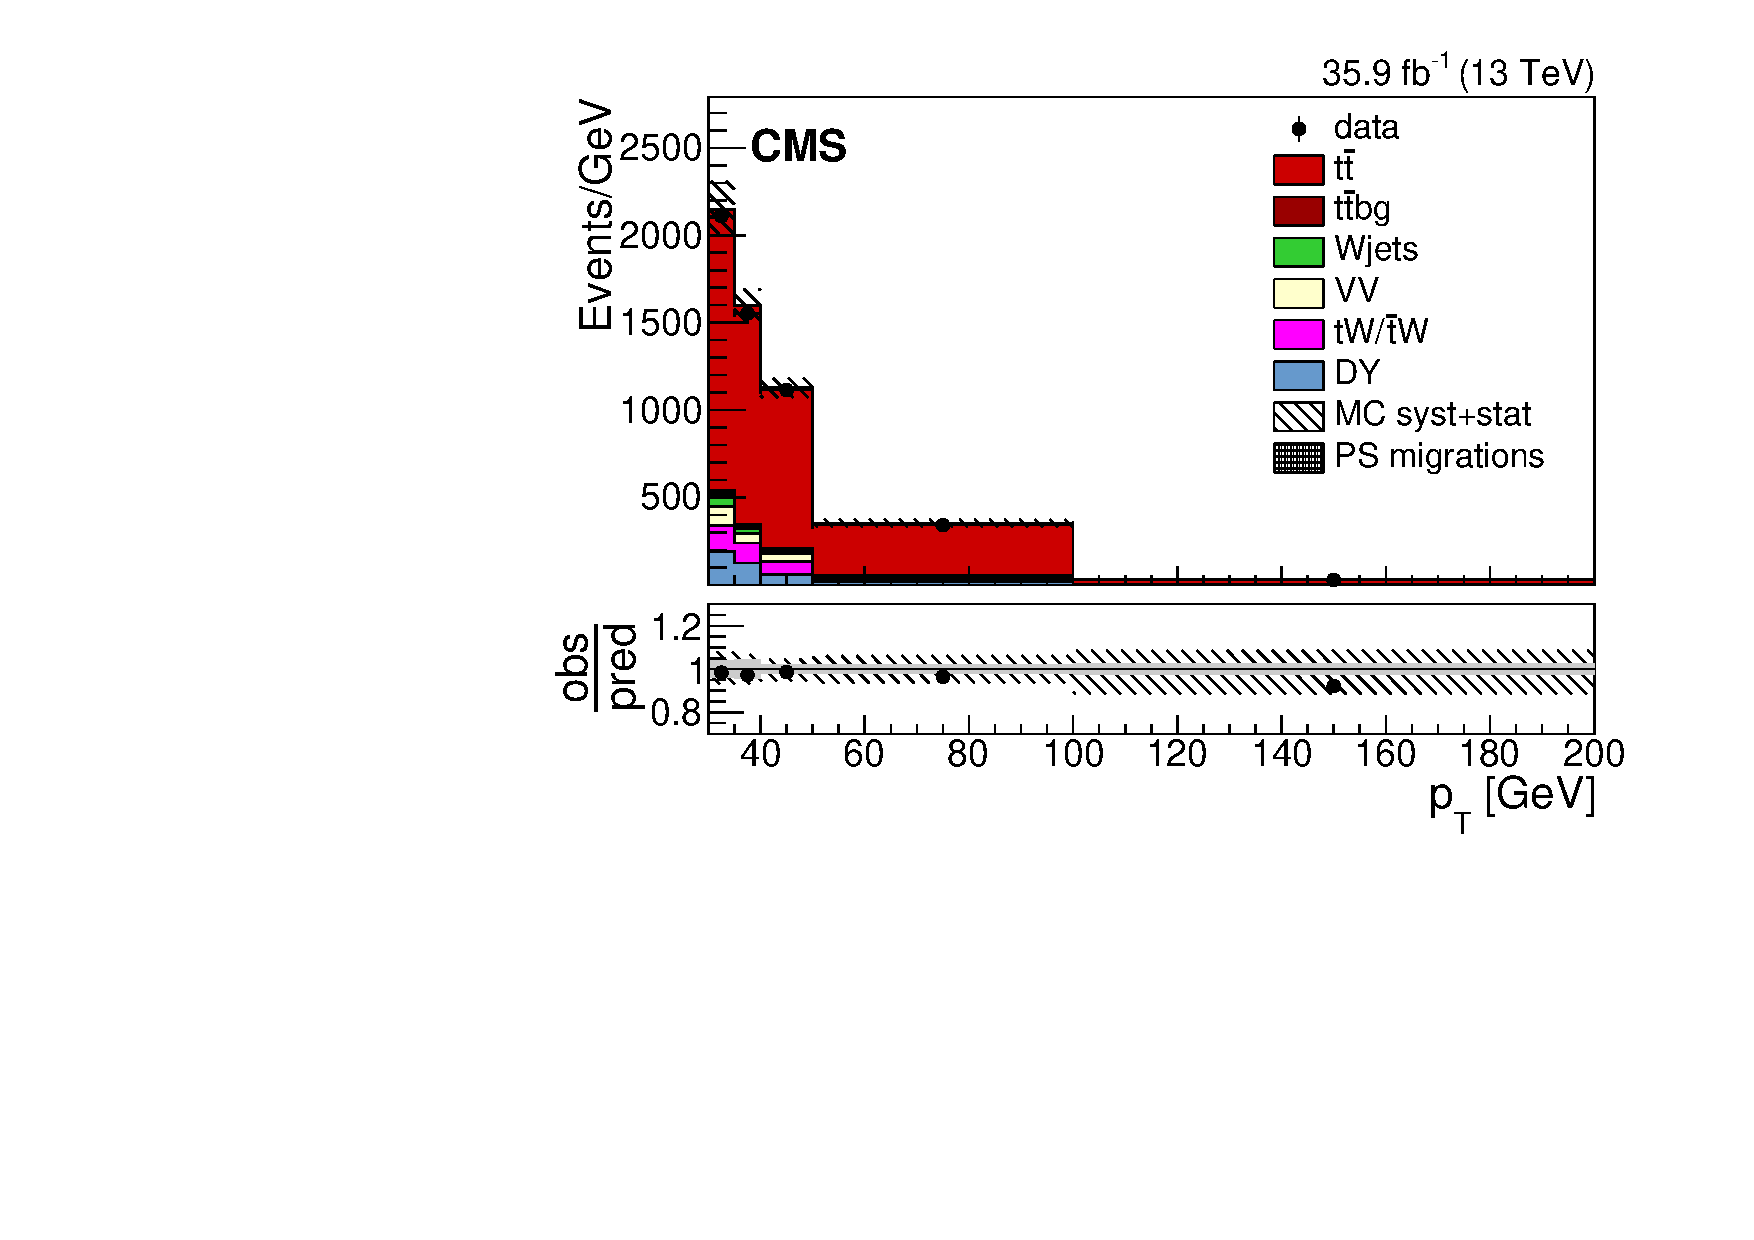
\includegraphics{CrossSection/Figures/ControlPlots/emu_sysnom/second_jet_pt_0_2_b-jets_step_8.pdf}}
    \resizebox{0.32 \textwidth}{!}{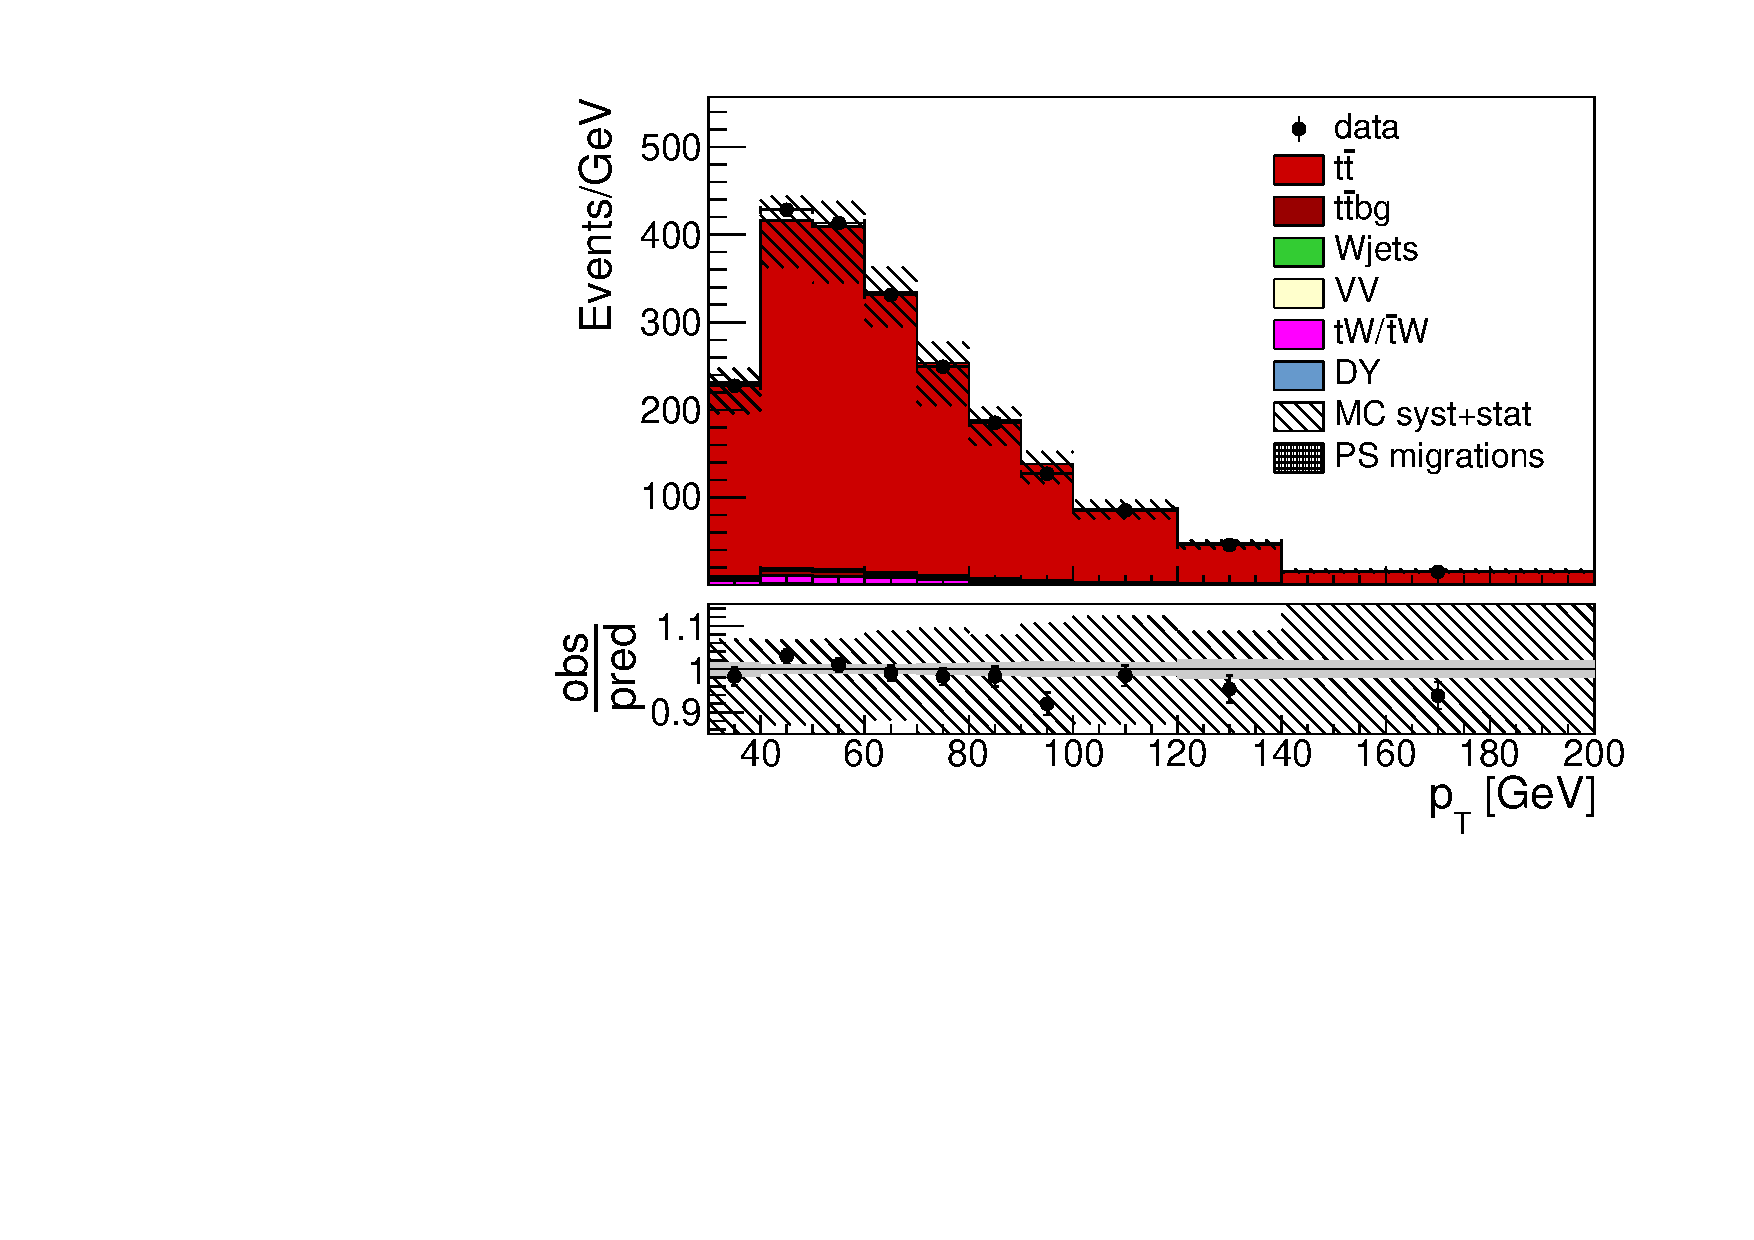
\includegraphics{CrossSection/Figures/ControlPlots/emu_sysnom/second_jet_pt_1_2_b-jets_step_8.pdf}}
    \resizebox{0.32 \textwidth}{!}{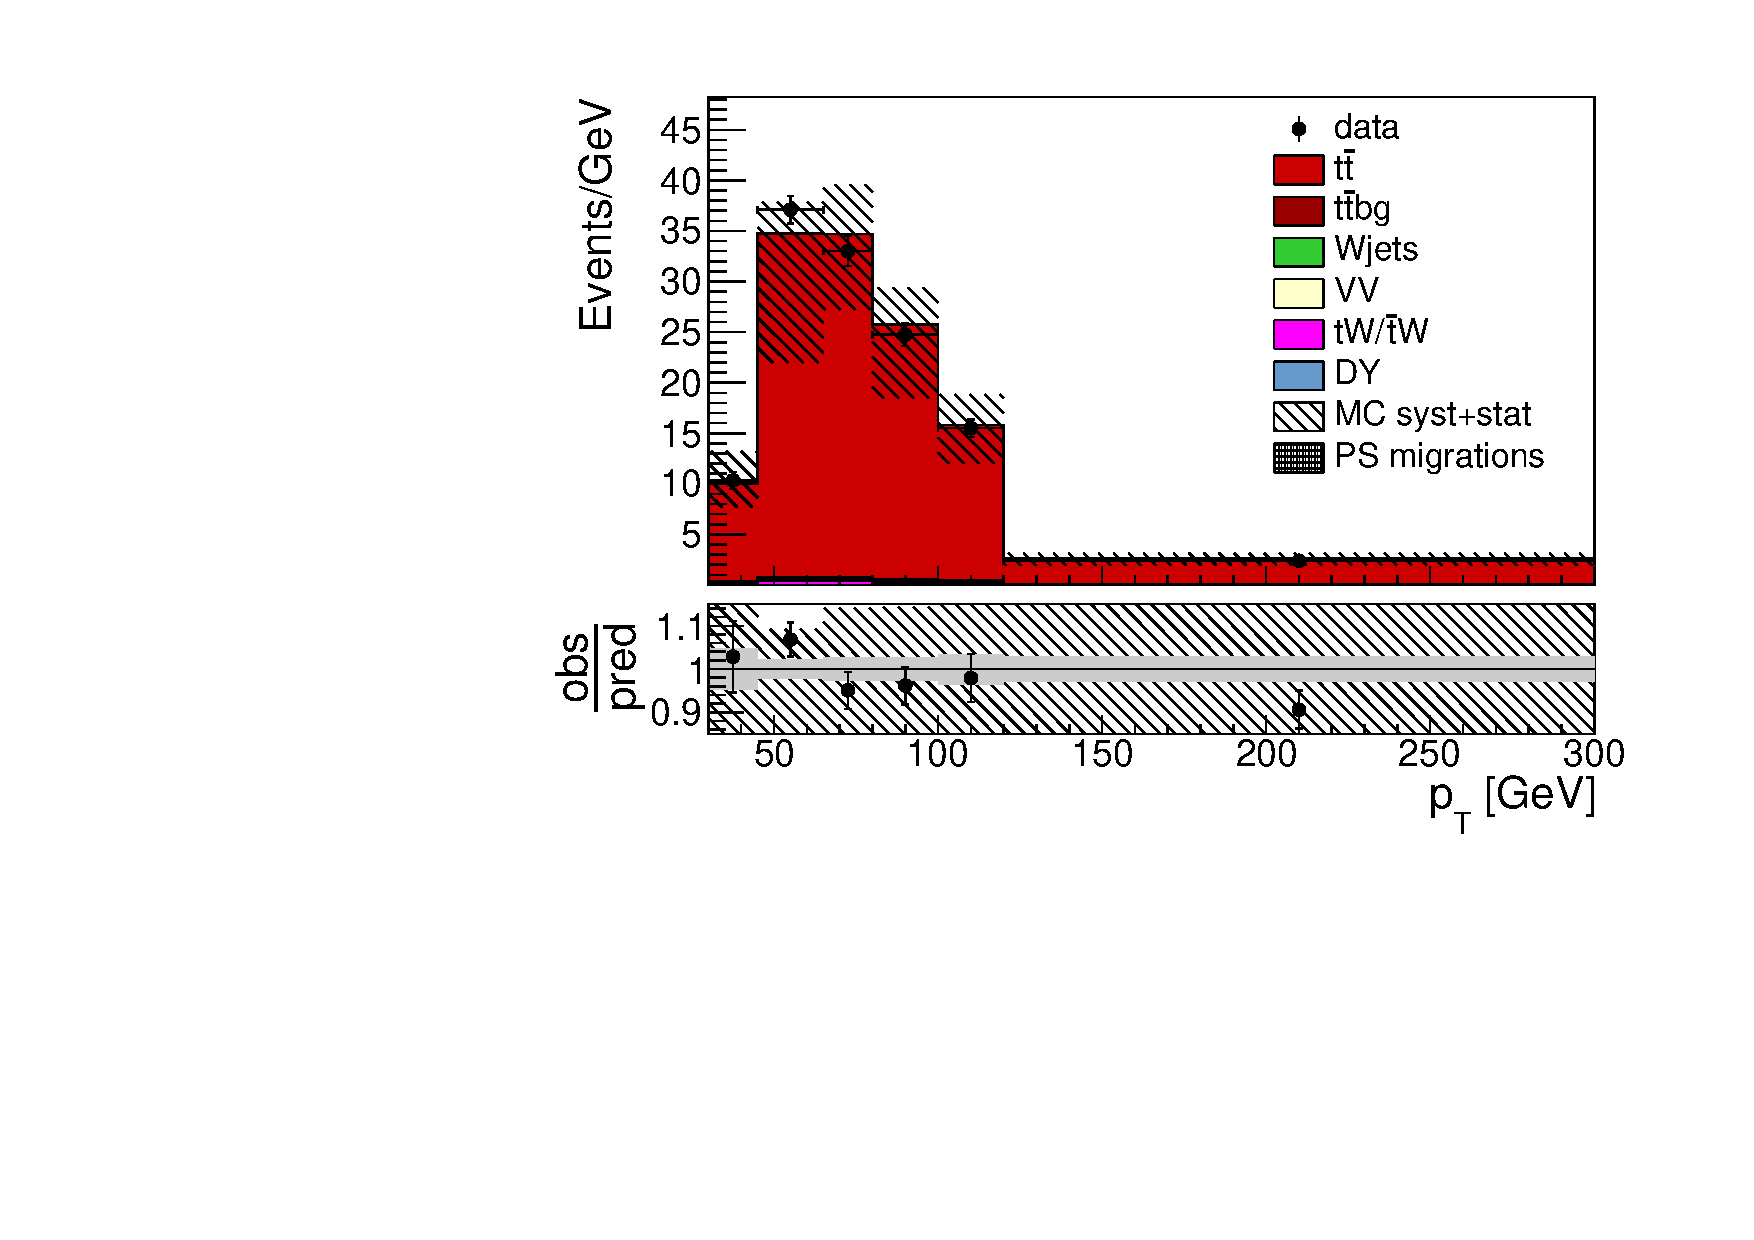
\includegraphics{CrossSection/Figures/ControlPlots/emu_sysnom/second_jet_pt_2_2_b-jets_step_8.pdf}}

    \resizebox{0.32 \textwidth}{!}{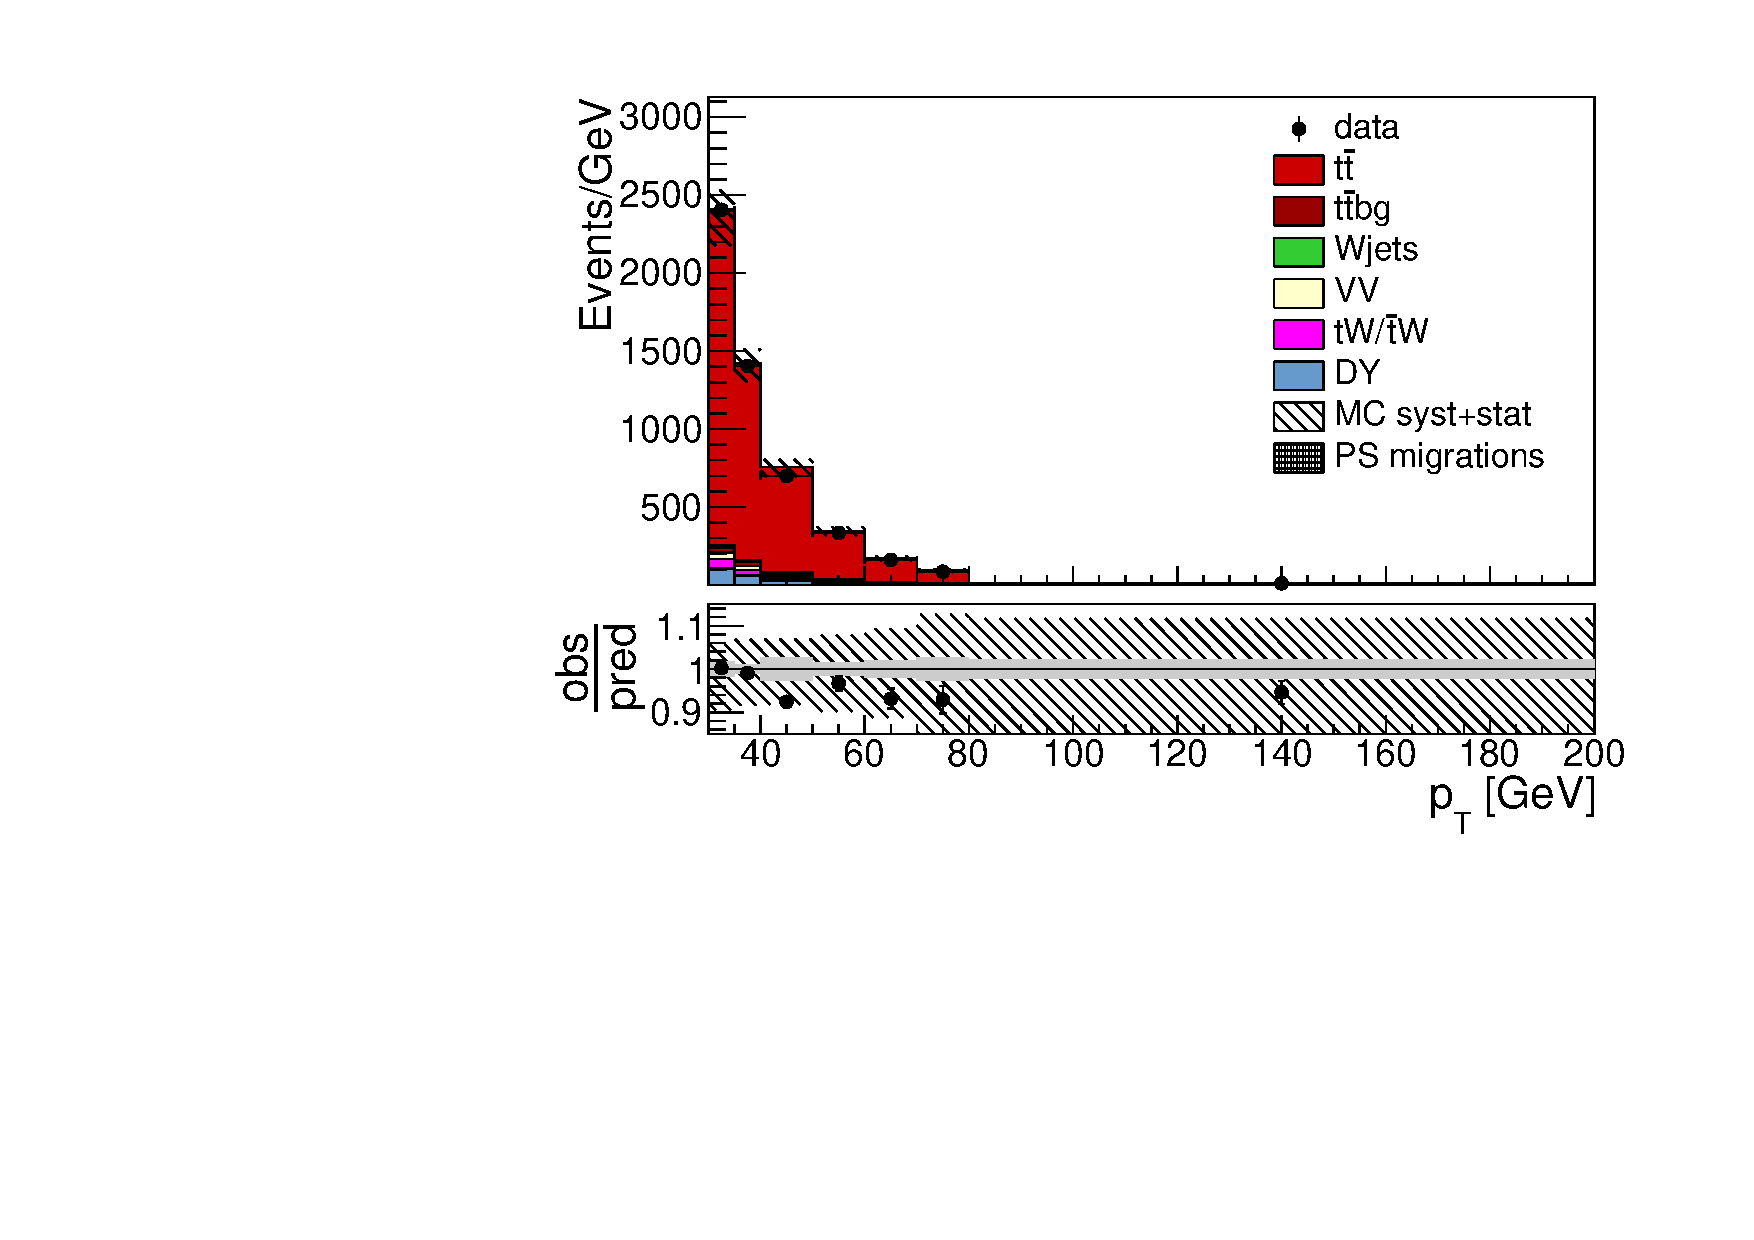
\includegraphics{CrossSection/Figures/ControlPlots/emu_sysnom/third_jet_pt_0_3_b-jets_step_8.pdf}}
    \resizebox{0.32 \textwidth}{!}{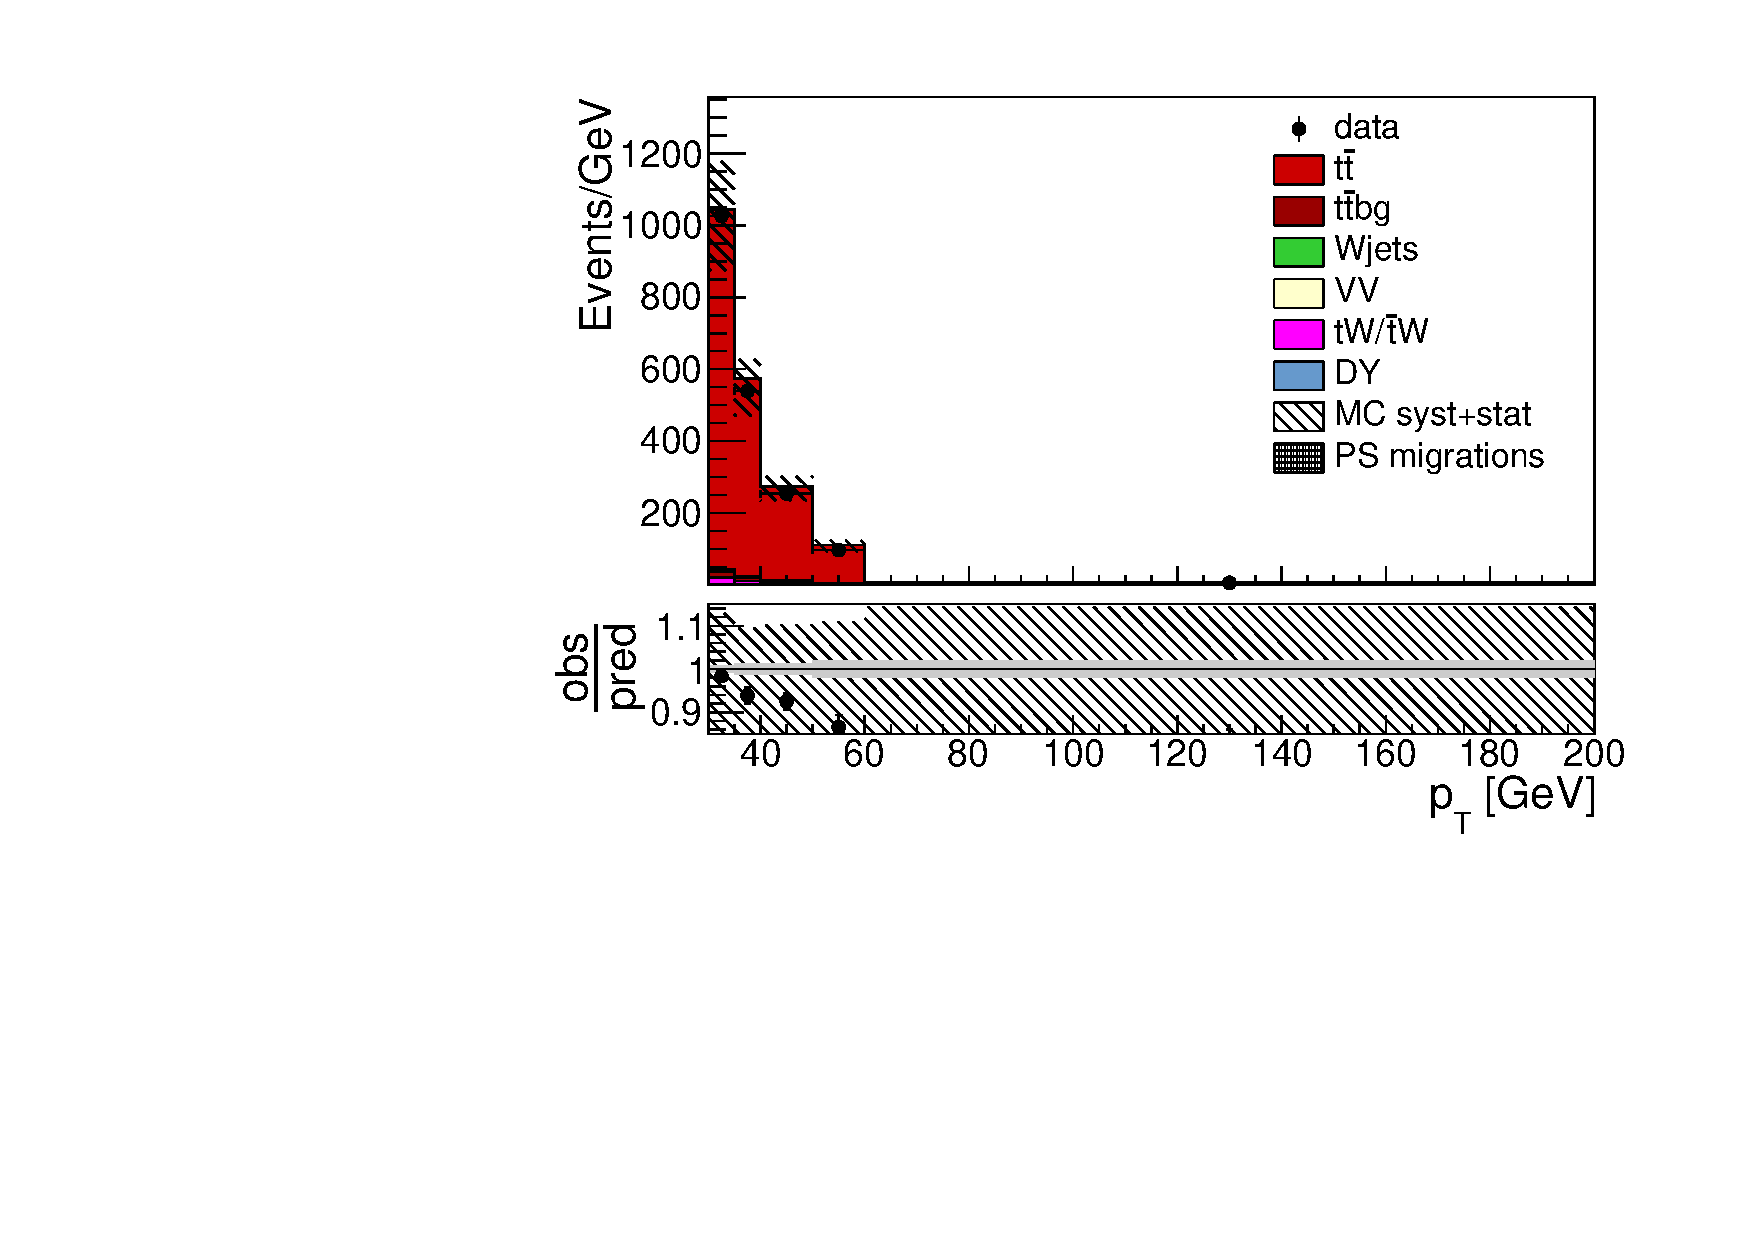
\includegraphics{CrossSection/Figures/ControlPlots/emu_sysnom/third_jet_pt_1_3_b-jets_step_8.pdf}}
    \resizebox{0.32 \textwidth}{!}{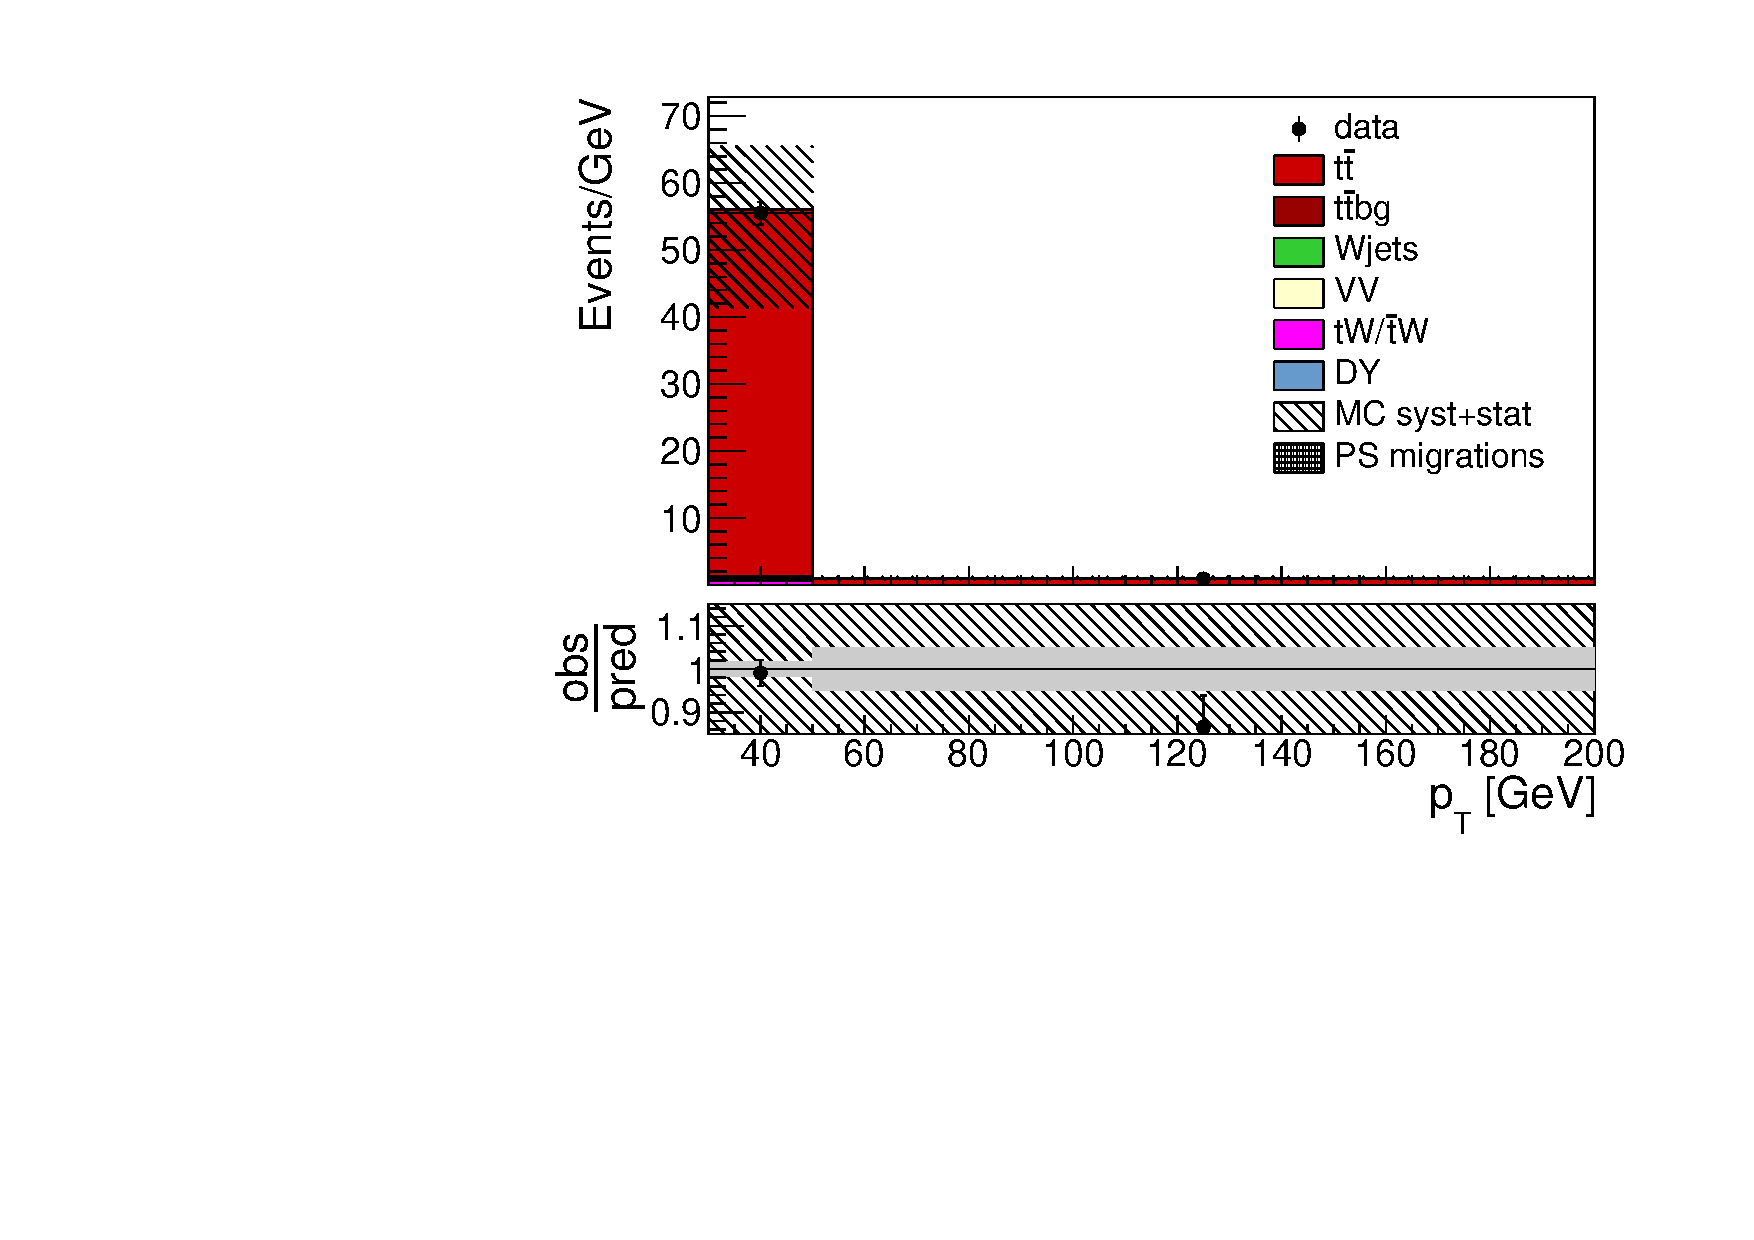
\includegraphics{CrossSection/Figures/ControlPlots/emu_sysnom/third_jet_pt_2_3_b-jets_step_8.pdf}}  

\caption{Pre-fit distributions (\emu channel) for events with zero as well as three or
  more b-tagged jets (left column): Total event yield for zero (top) and the trailing jet pt for one (second from top),
  two (second from bottom) or three or more (bottom) additional jets. The same for events with one
  b-tagged jet (middle column) and two b-tagged jets (right column) are
  shown below.   
  The hatched bands correspond to the total uncertainty on the sum of
  the predicted yields. The ratios of data to the sum of the
  predicted yields are shown at the bottom of each plot. Here, the solid
  gray band represents the contribution of the statistical uncertainty.  
       \label{fig:xsec_emu_inputdistr}}
  \end{center}
\end{figure}

\begin{figure}[htbp!]
  \begin{center}
    \resizebox{0.240 \textwidth}{!}{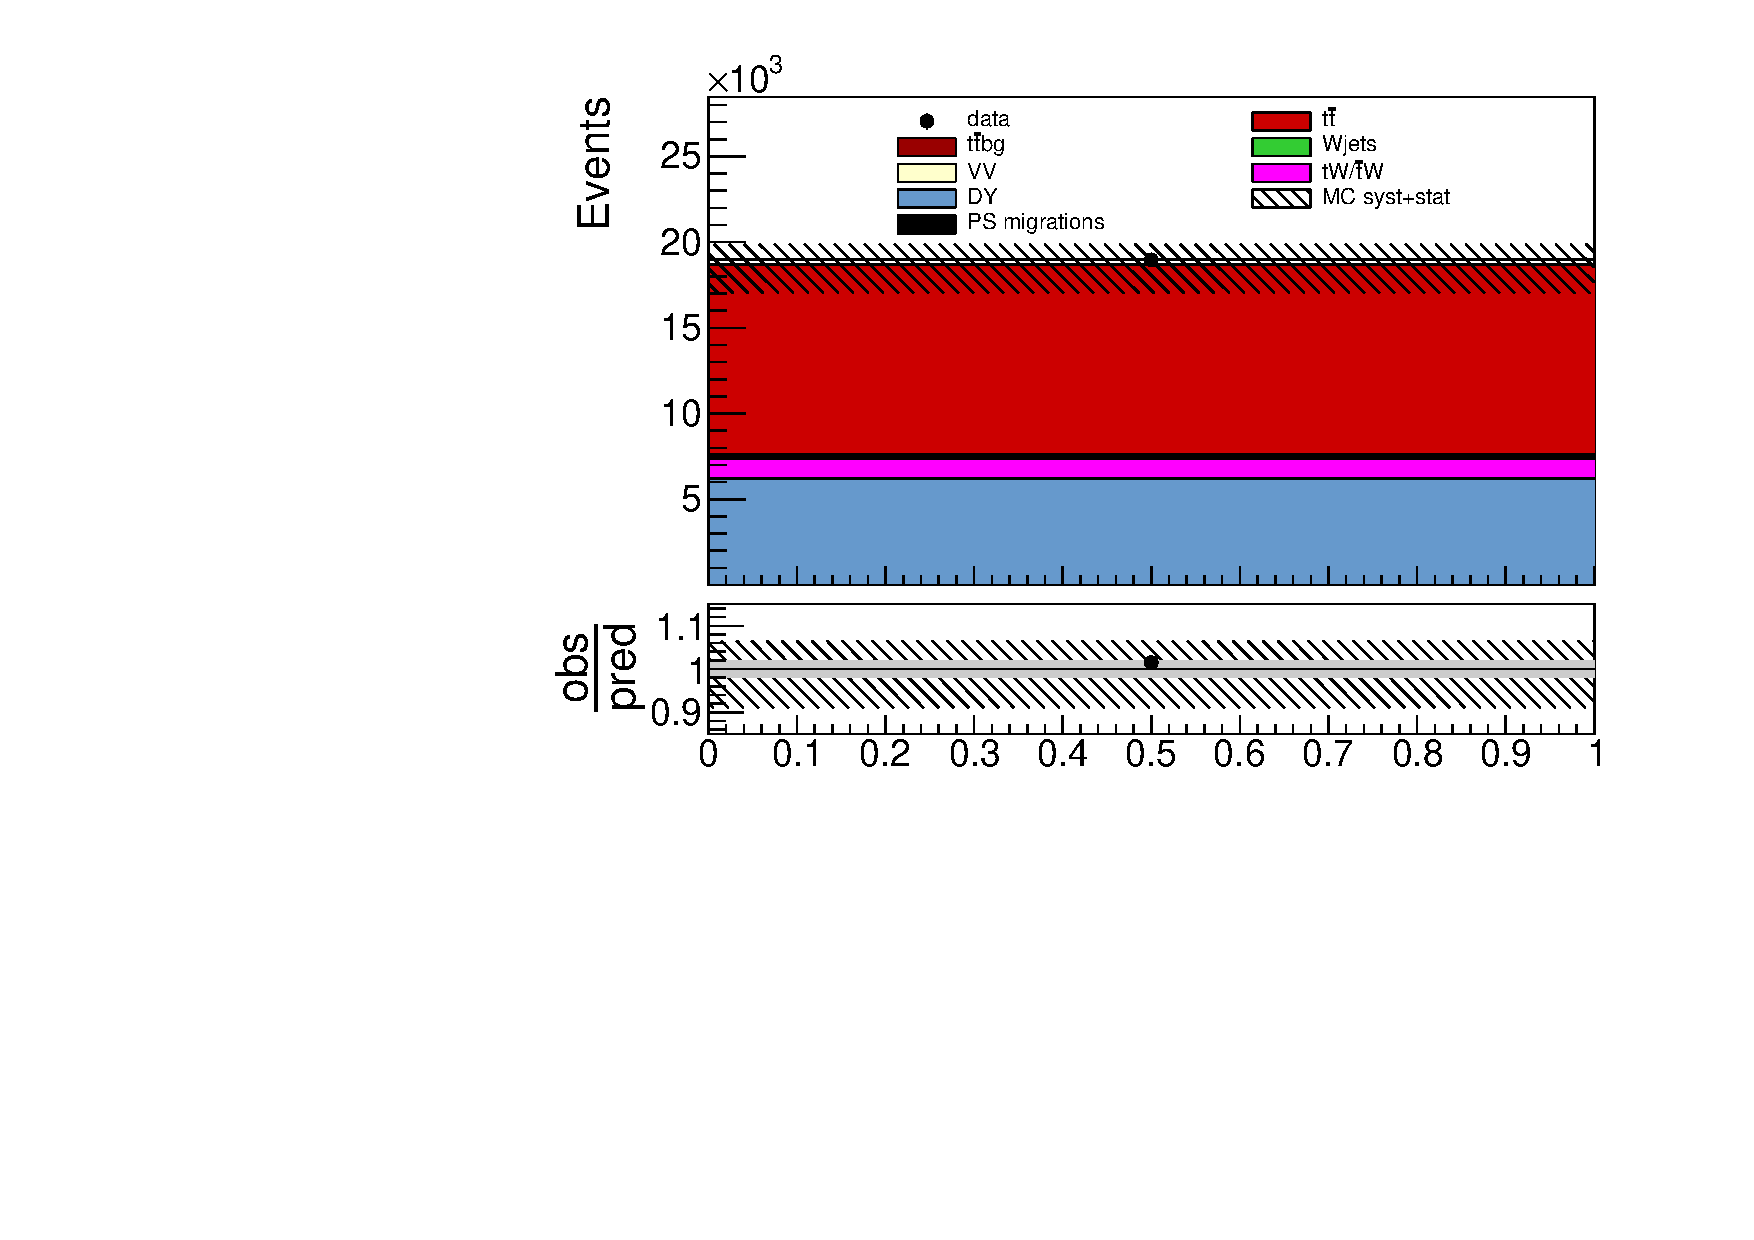
\includegraphics{CrossSection/Figures/ControlPlots/mumu_sysnom/total_1_0_b-jets_step_8.pdf}}
    \resizebox{0.240 \textwidth}{!}{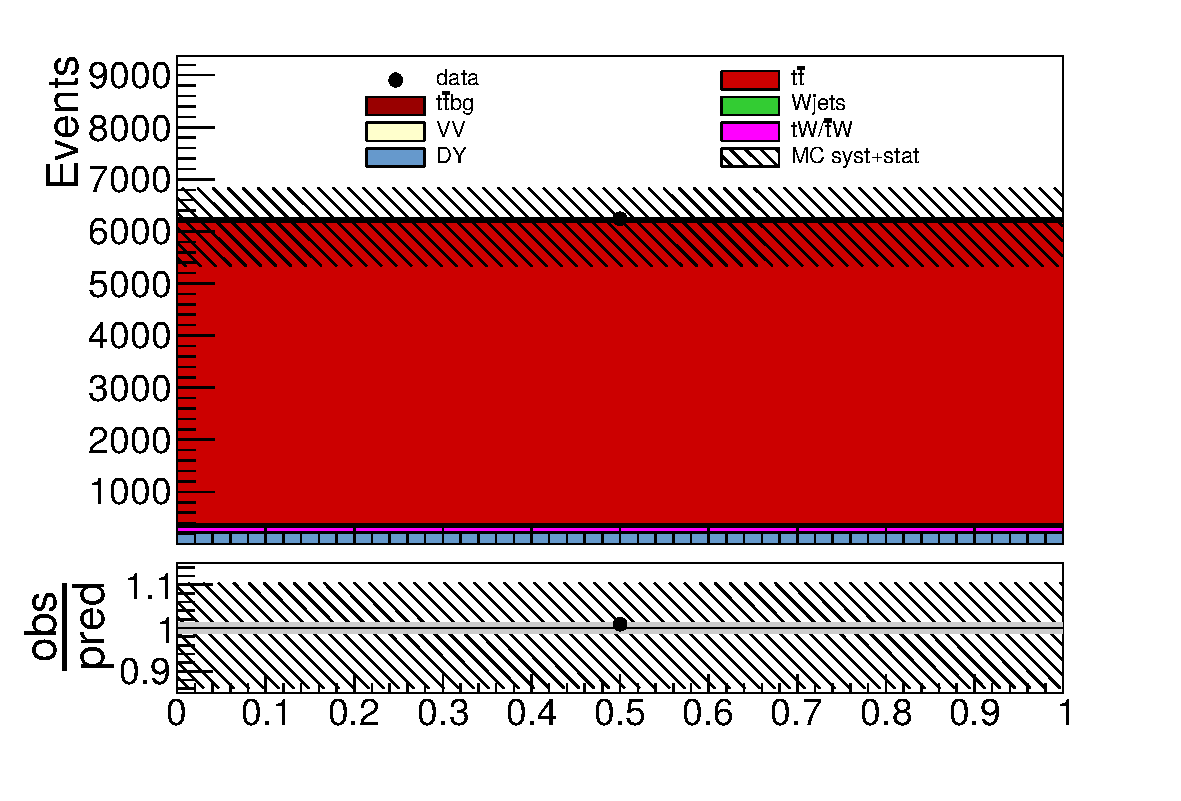
\includegraphics{CrossSection/Figures/ControlPlots/mumu_sysnom/total_2_0_b-jets_step_8.pdf}} \\

    \resizebox{0.40 \textwidth}{!}{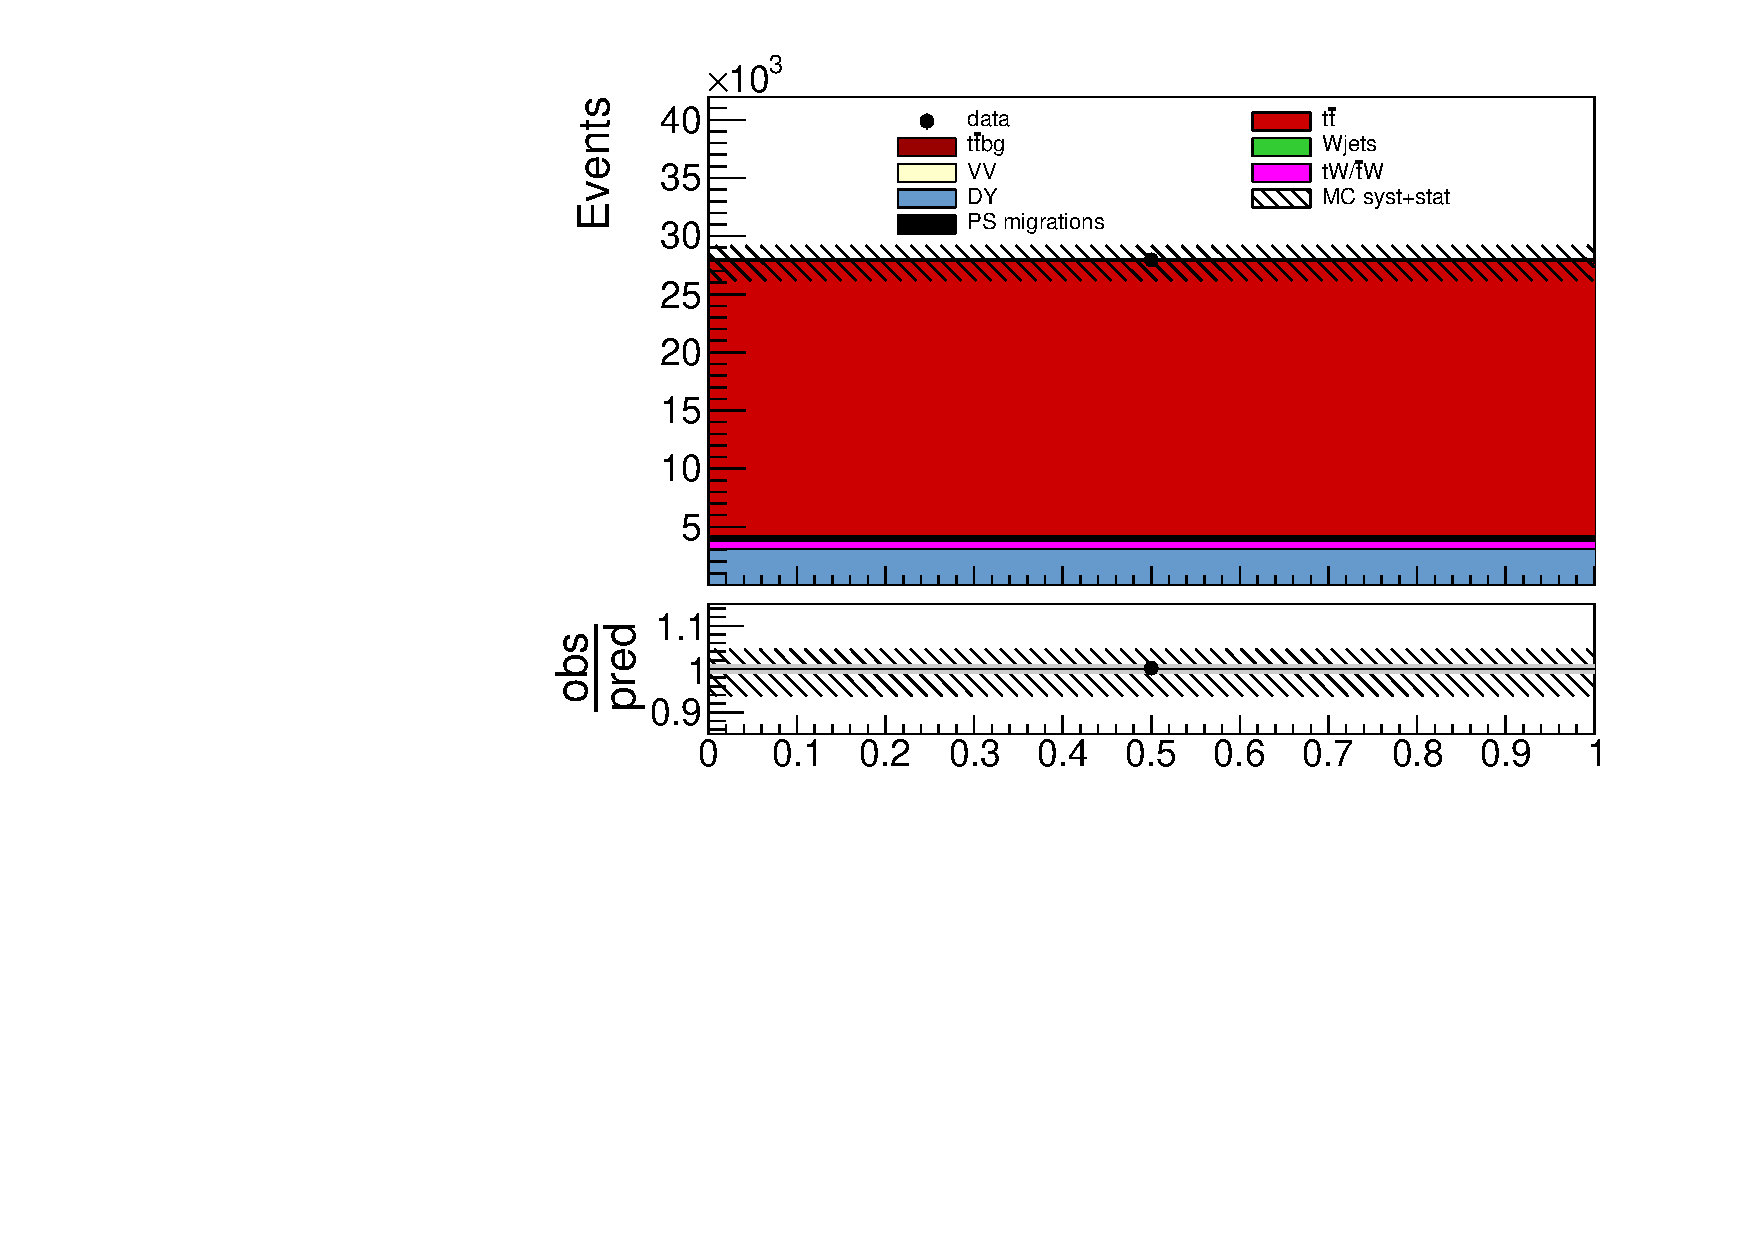
\includegraphics{CrossSection/Figures/ControlPlots/mumu_sysnom/total_1_1_b-jets_step_8.pdf}}
    \resizebox{0.40 \textwidth}{!}{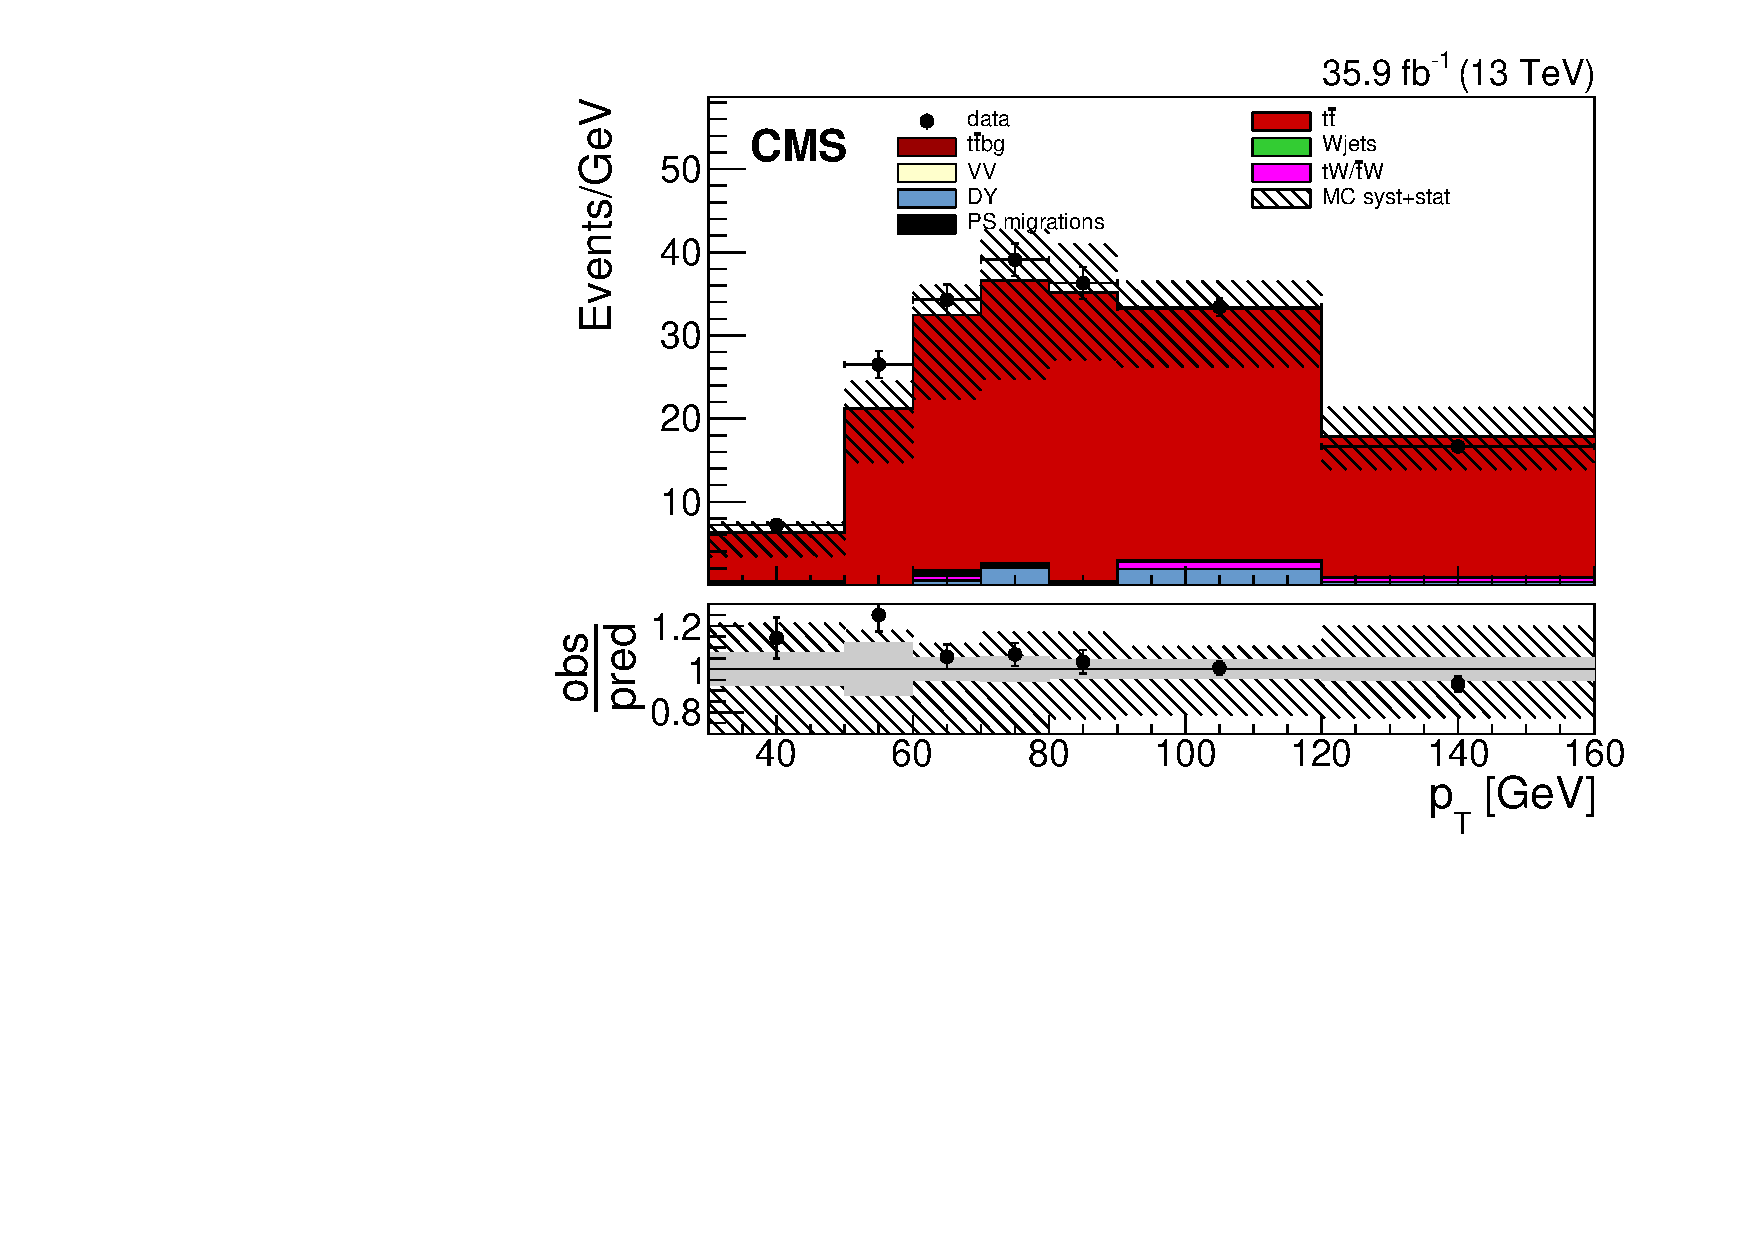
\includegraphics{CrossSection/Figures/ControlPlots/mumu_sysnom/lead_jet_pt_2_1_b-jets_step_8.pdf}}\\
        
    \resizebox{0.4 \textwidth}{!}{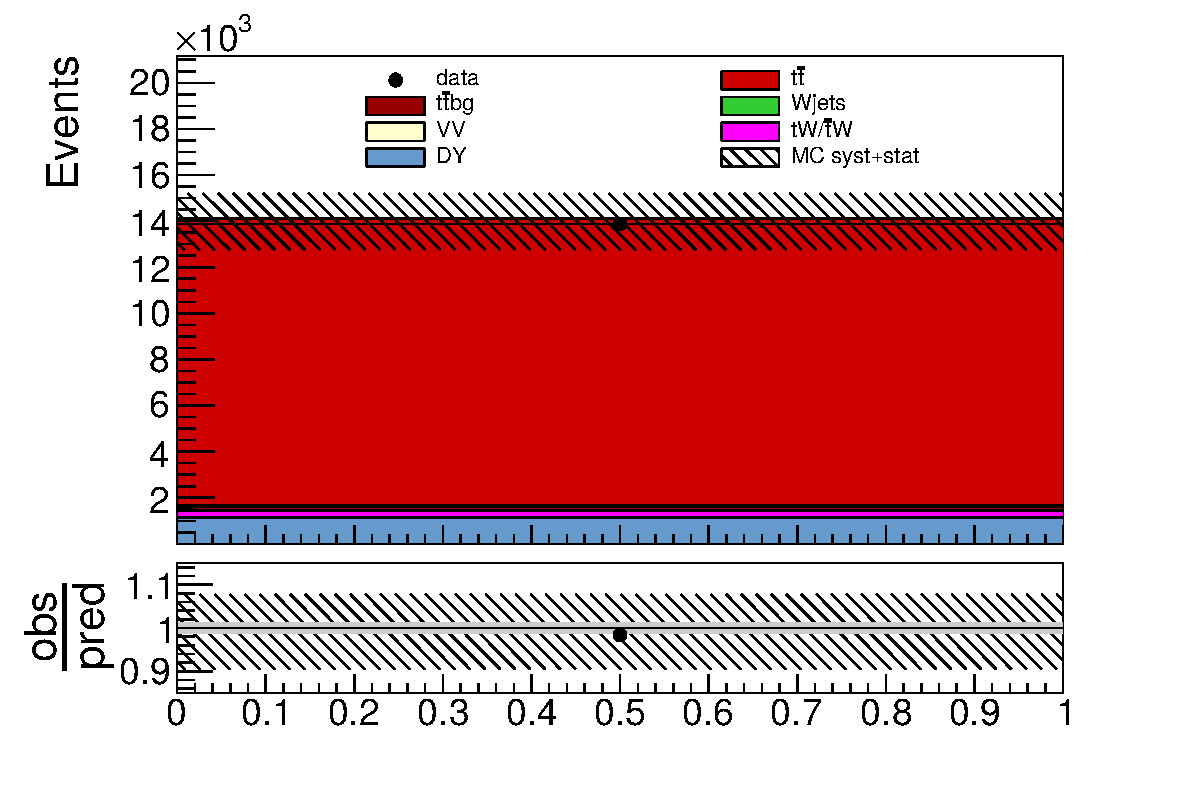
\includegraphics{CrossSection/Figures/ControlPlots/mumu_sysnom/total_1_2_b-jets_step_8.pdf}}
    \resizebox{0.4 \textwidth}{!}{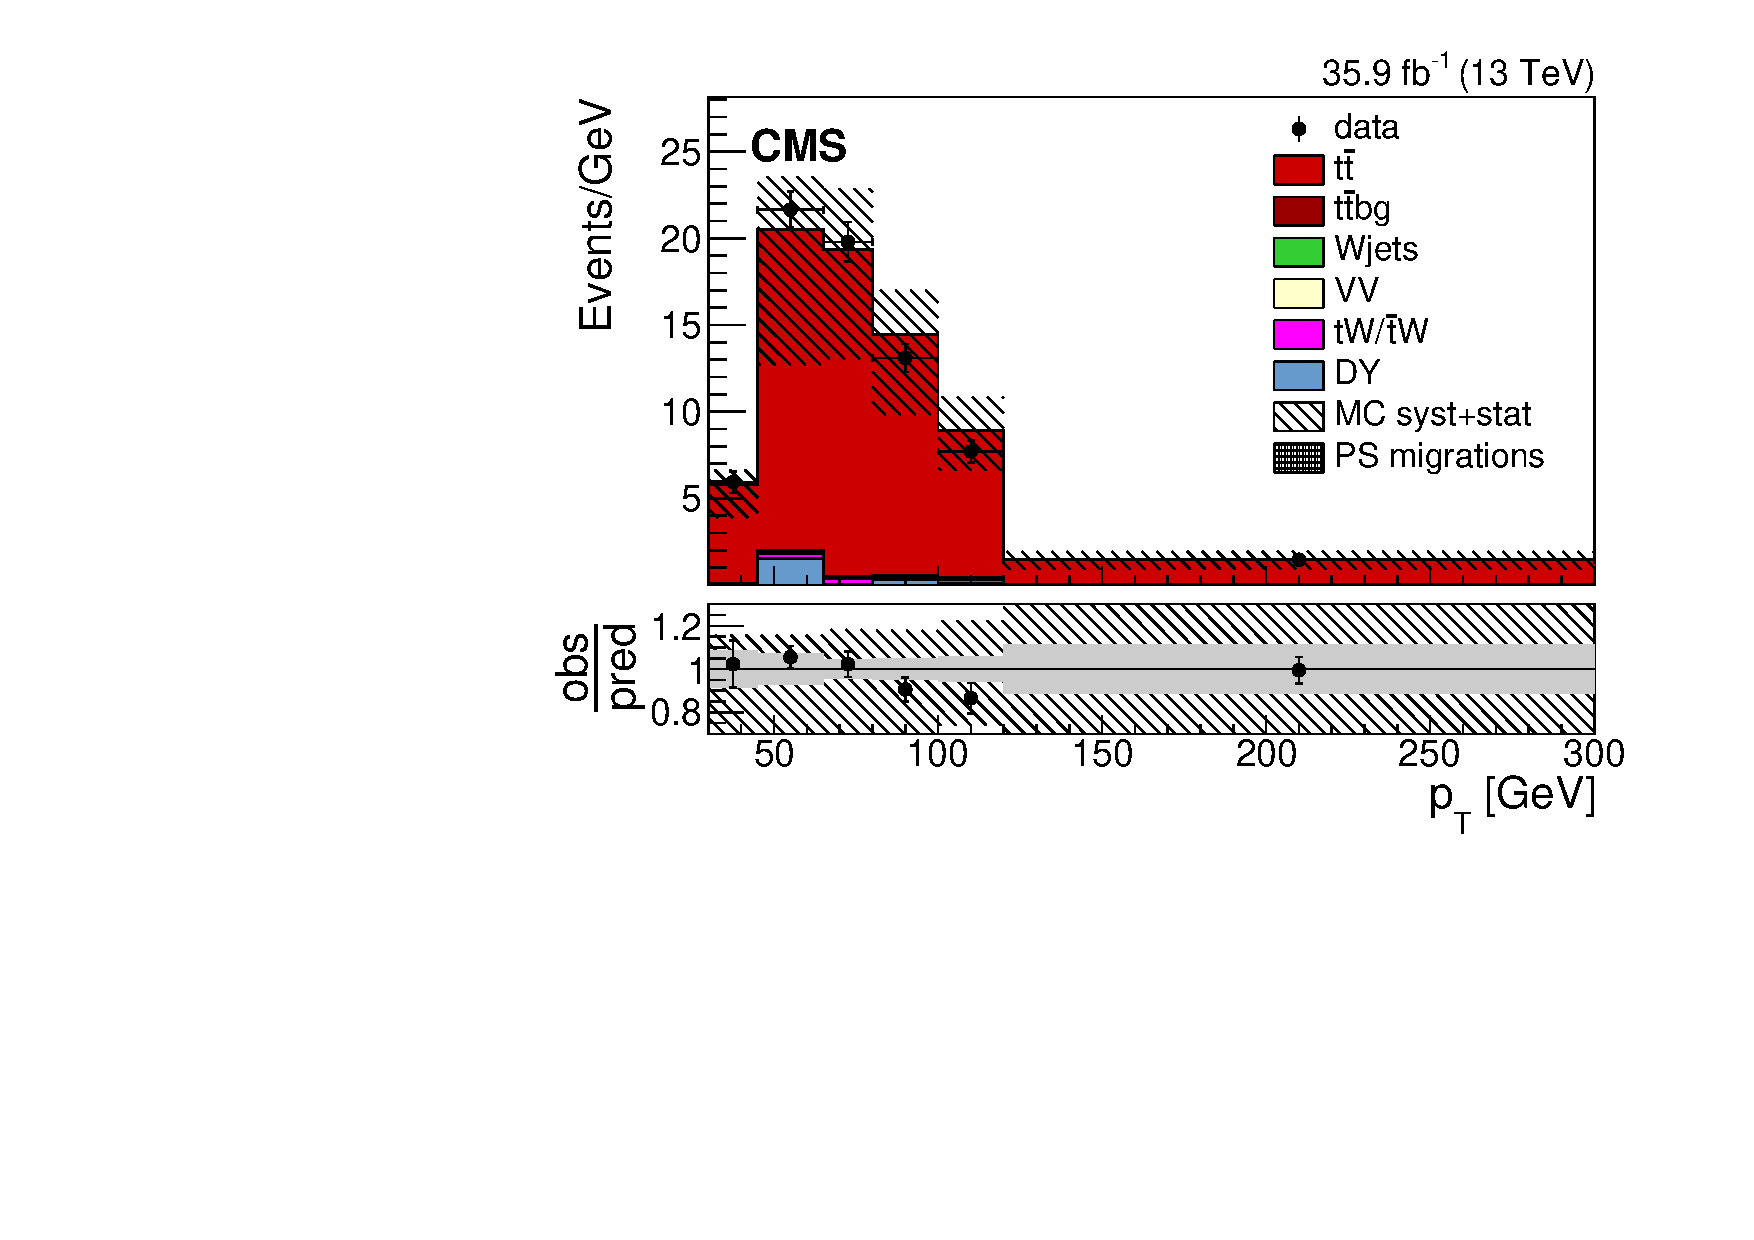
\includegraphics{CrossSection/Figures/ControlPlots/mumu_sysnom/second_jet_pt_2_2_b-jets_step_8.pdf}}\\

    \resizebox{0.4 \textwidth}{!}{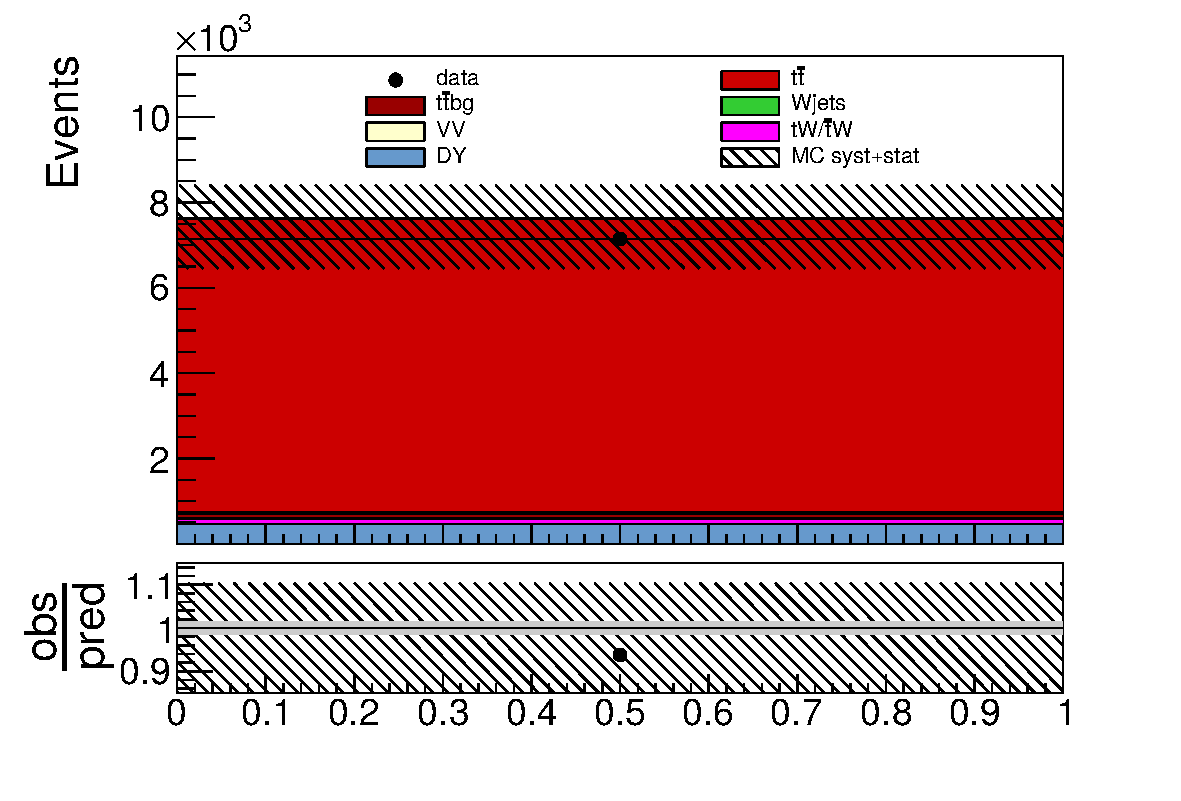
\includegraphics{CrossSection/Figures/ControlPlots/mumu_sysnom/total_1_3_b-jets_step_8.pdf}}
    \resizebox{0.4 \textwidth}{!}{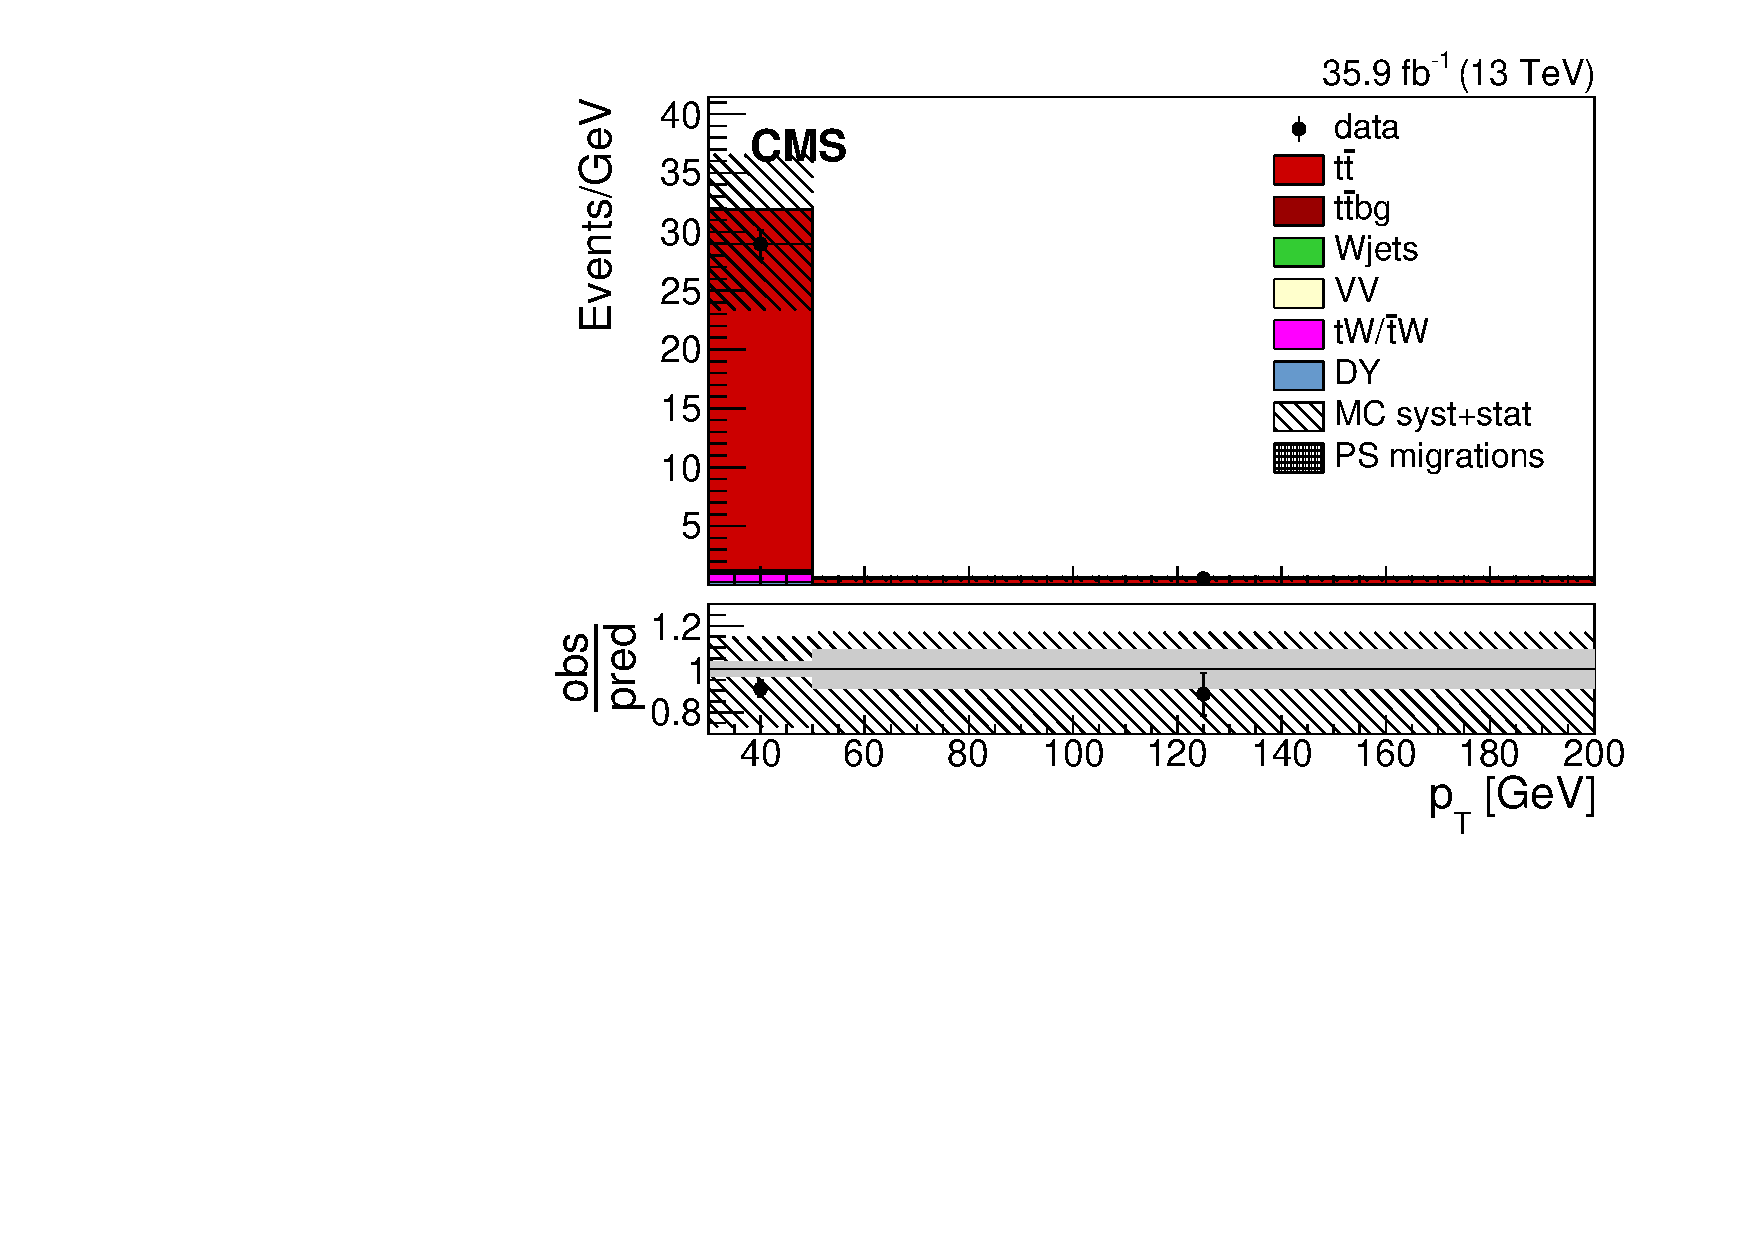
\includegraphics{CrossSection/Figures/ControlPlots/mumu_sysnom/third_jet_pt_2_3_b-jets_step_8.pdf}}  
\caption{Pre-fit distributions (\mumu channel): 
  The left column shows events with one b-tagged jet and the total event yield for events with zero (top), one (second from top)
  two (second from bottom) or three or more additional jets (bottom).
  The right column shows events with two b-tagged jets and the total yield for events with zero additional jets (top),
  the trailing jet pt for one (second from top),
  two (second from bottom) or three or more (bottom) additional jets.
  The hatched bands correspond to the total uncertainty on the sum of
  the predicted yields. The ratios of data to the sum of the
  predicted yields are shown at the bottom of each plot. Here, the solid
  gray band represents the contribution of the statistical uncertainty.  
       \label{fig:xsec_mumu_inputdistr}}
  \end{center}
\end{figure}

\begin{figure}[htbp!]
  \begin{center}
    \resizebox{0.24 \textwidth}{!}{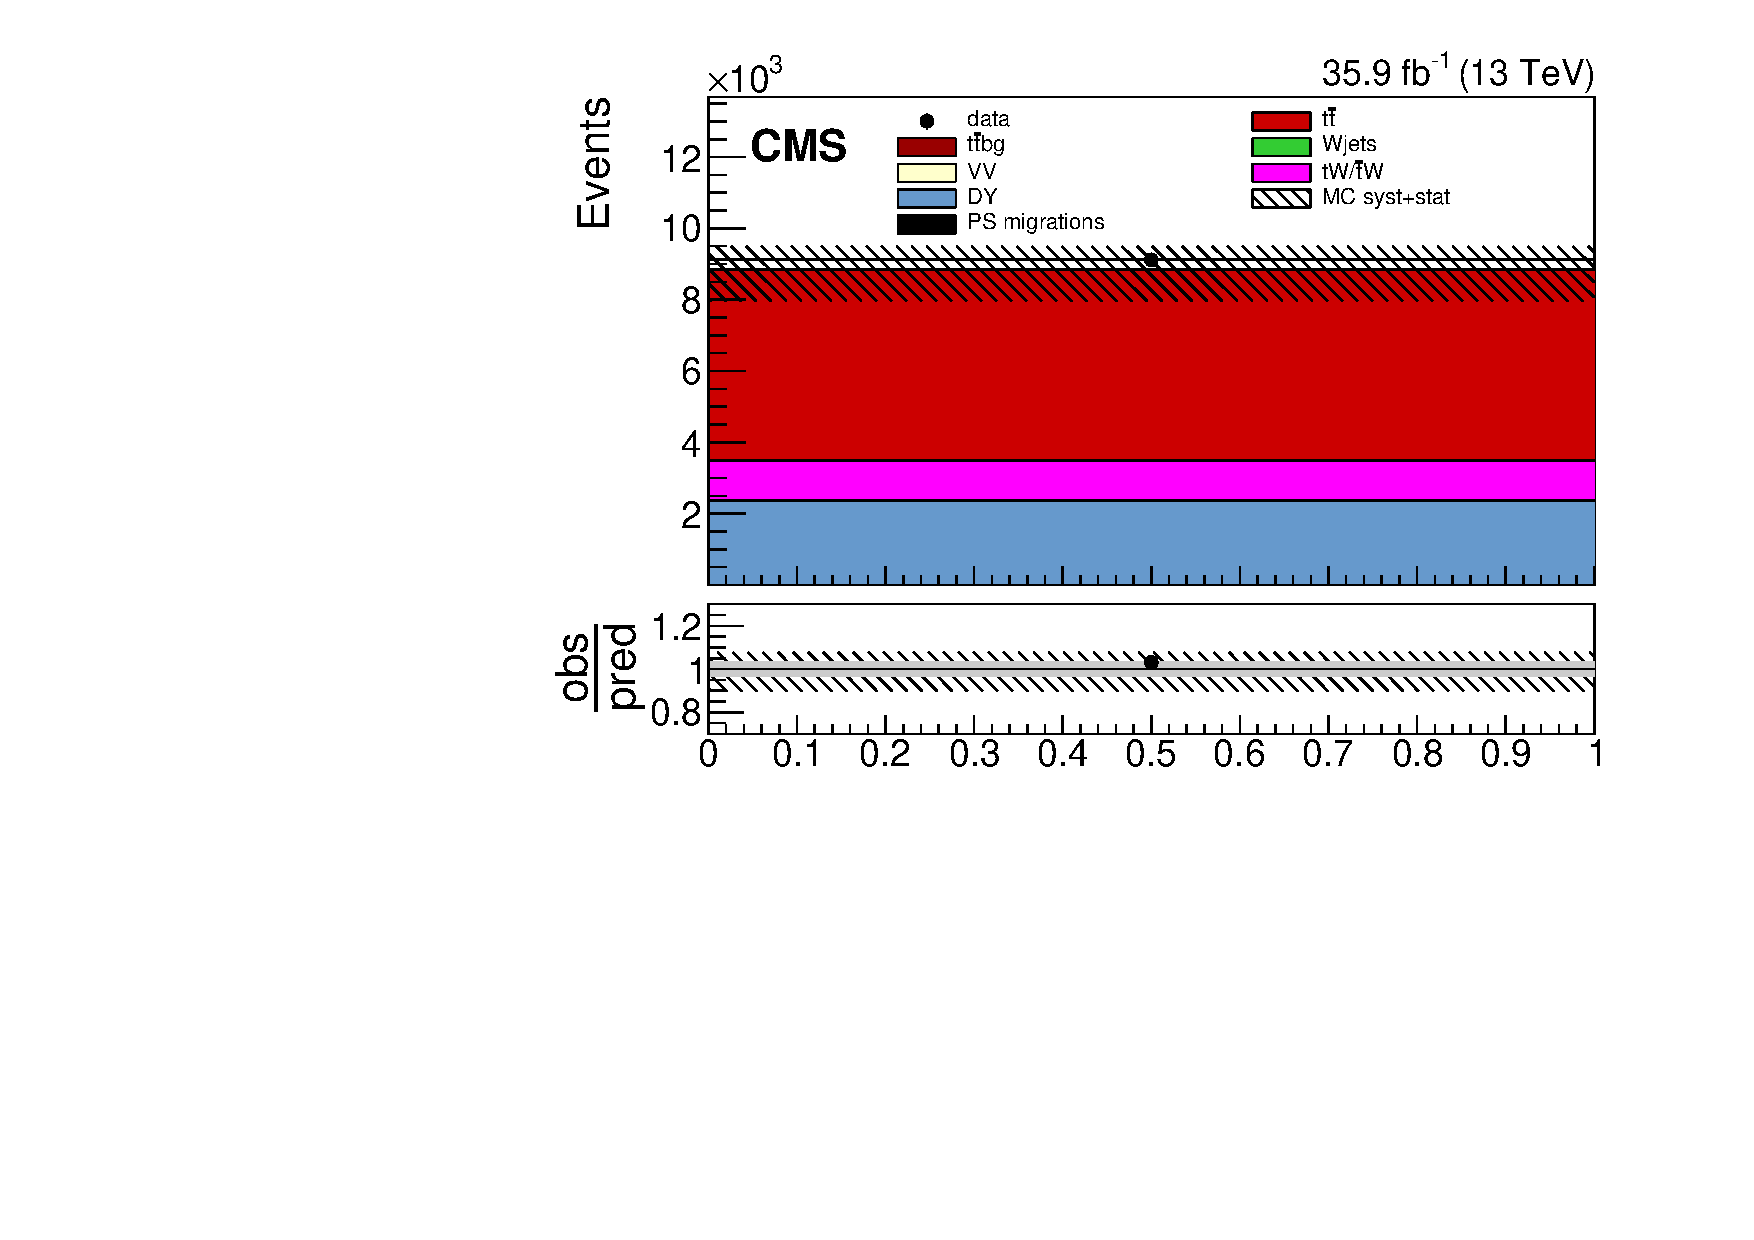
\includegraphics{CrossSection/Figures/ControlPlots/ee_sysnom/total_1_0_b-jets_step_8.pdf}}
    \resizebox{0.24 \textwidth}{!}{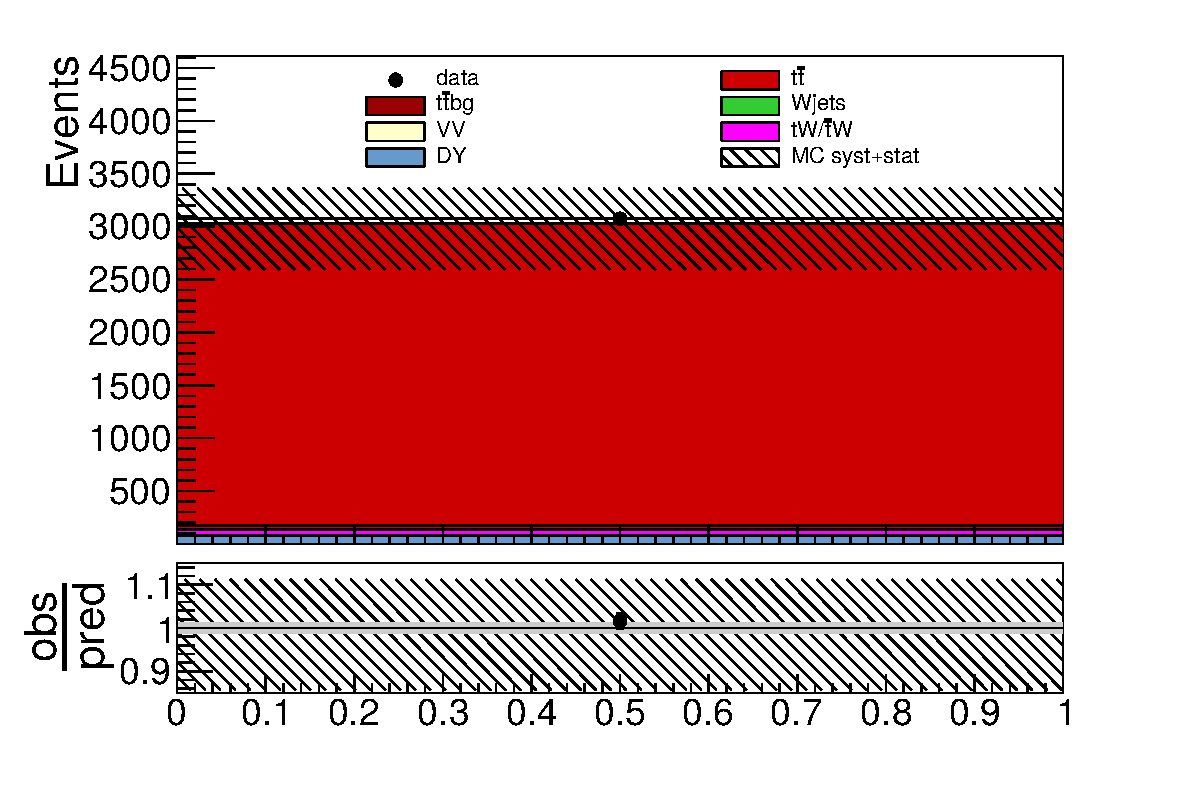
\includegraphics{CrossSection/Figures/ControlPlots/ee_sysnom/total_2_0_b-jets_step_8.pdf}}\\

    \resizebox{0.4 \textwidth}{!}{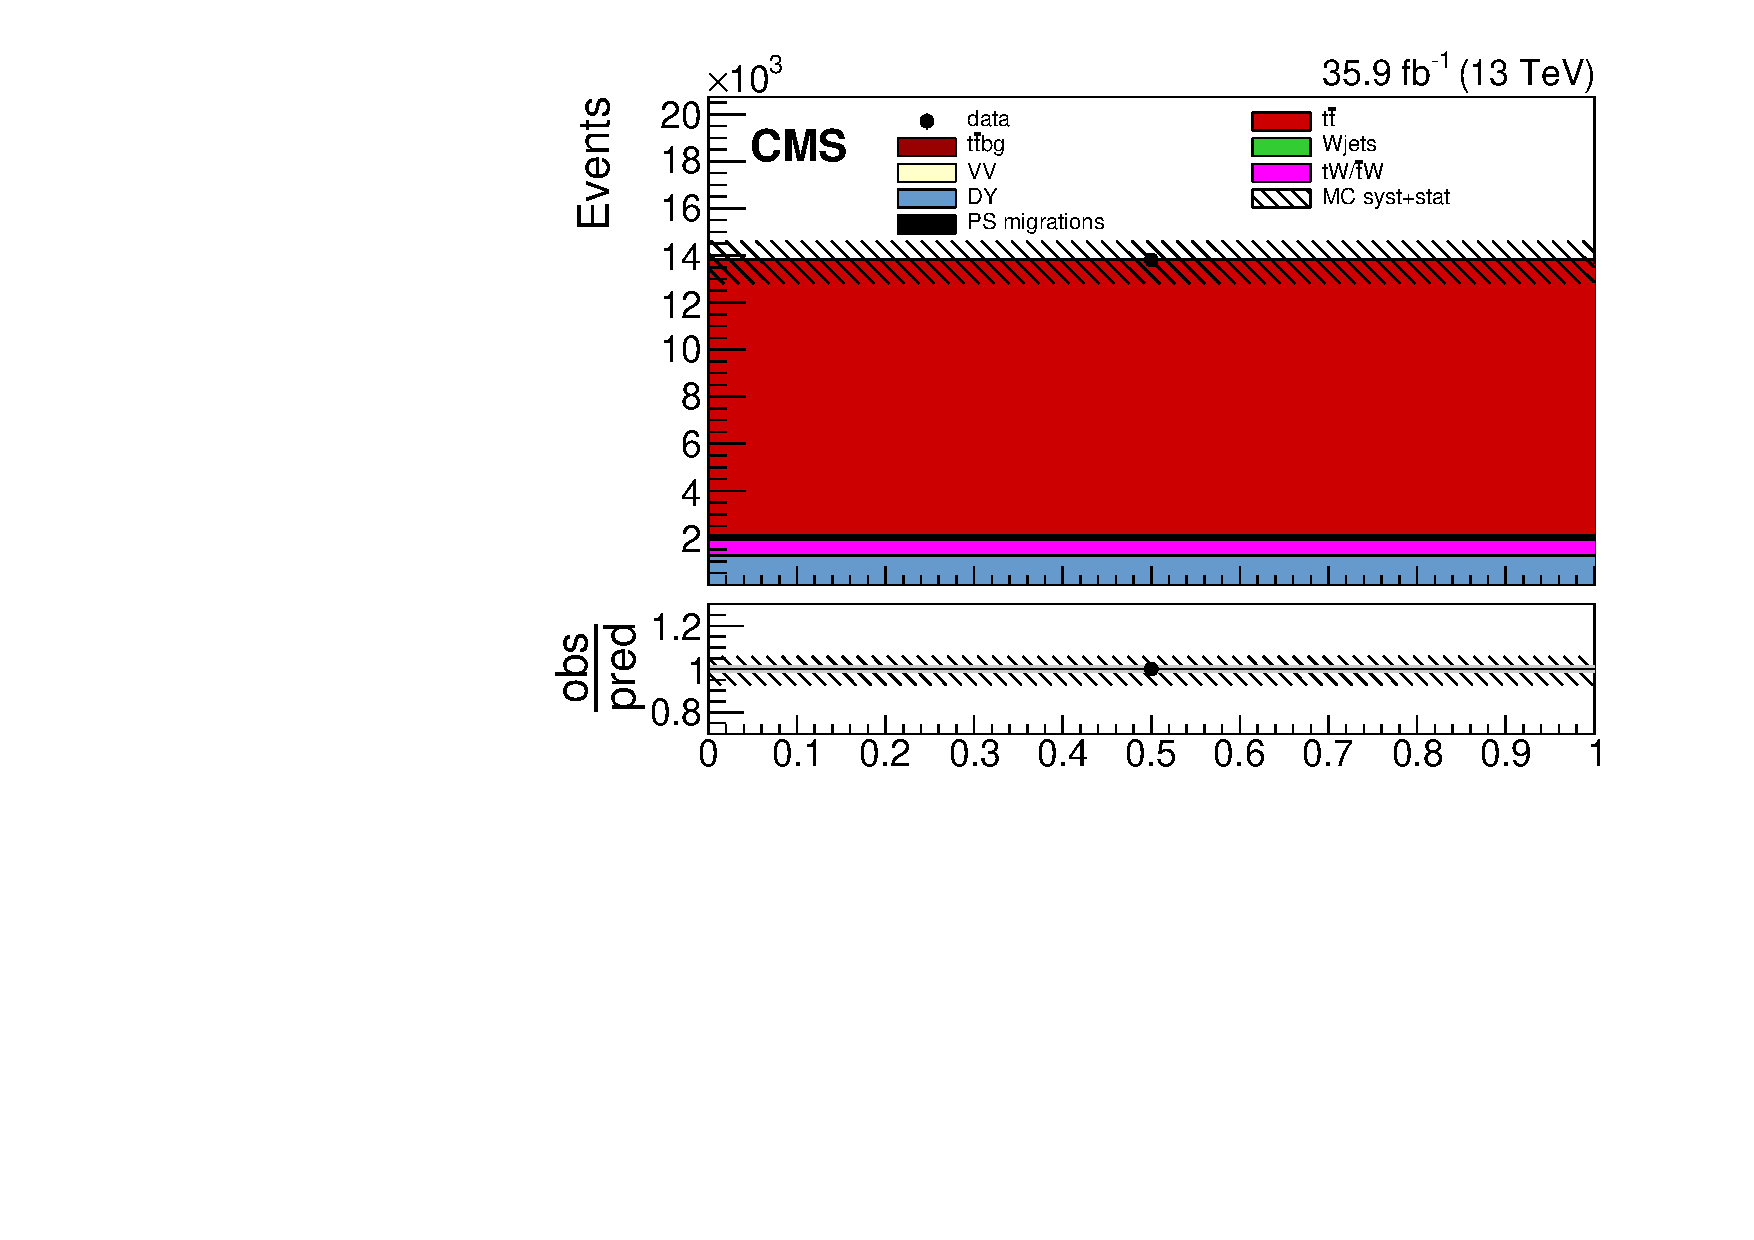
\includegraphics{CrossSection/Figures/ControlPlots/ee_sysnom/total_1_1_b-jets_step_8.pdf}}
    \resizebox{0.4 \textwidth}{!}{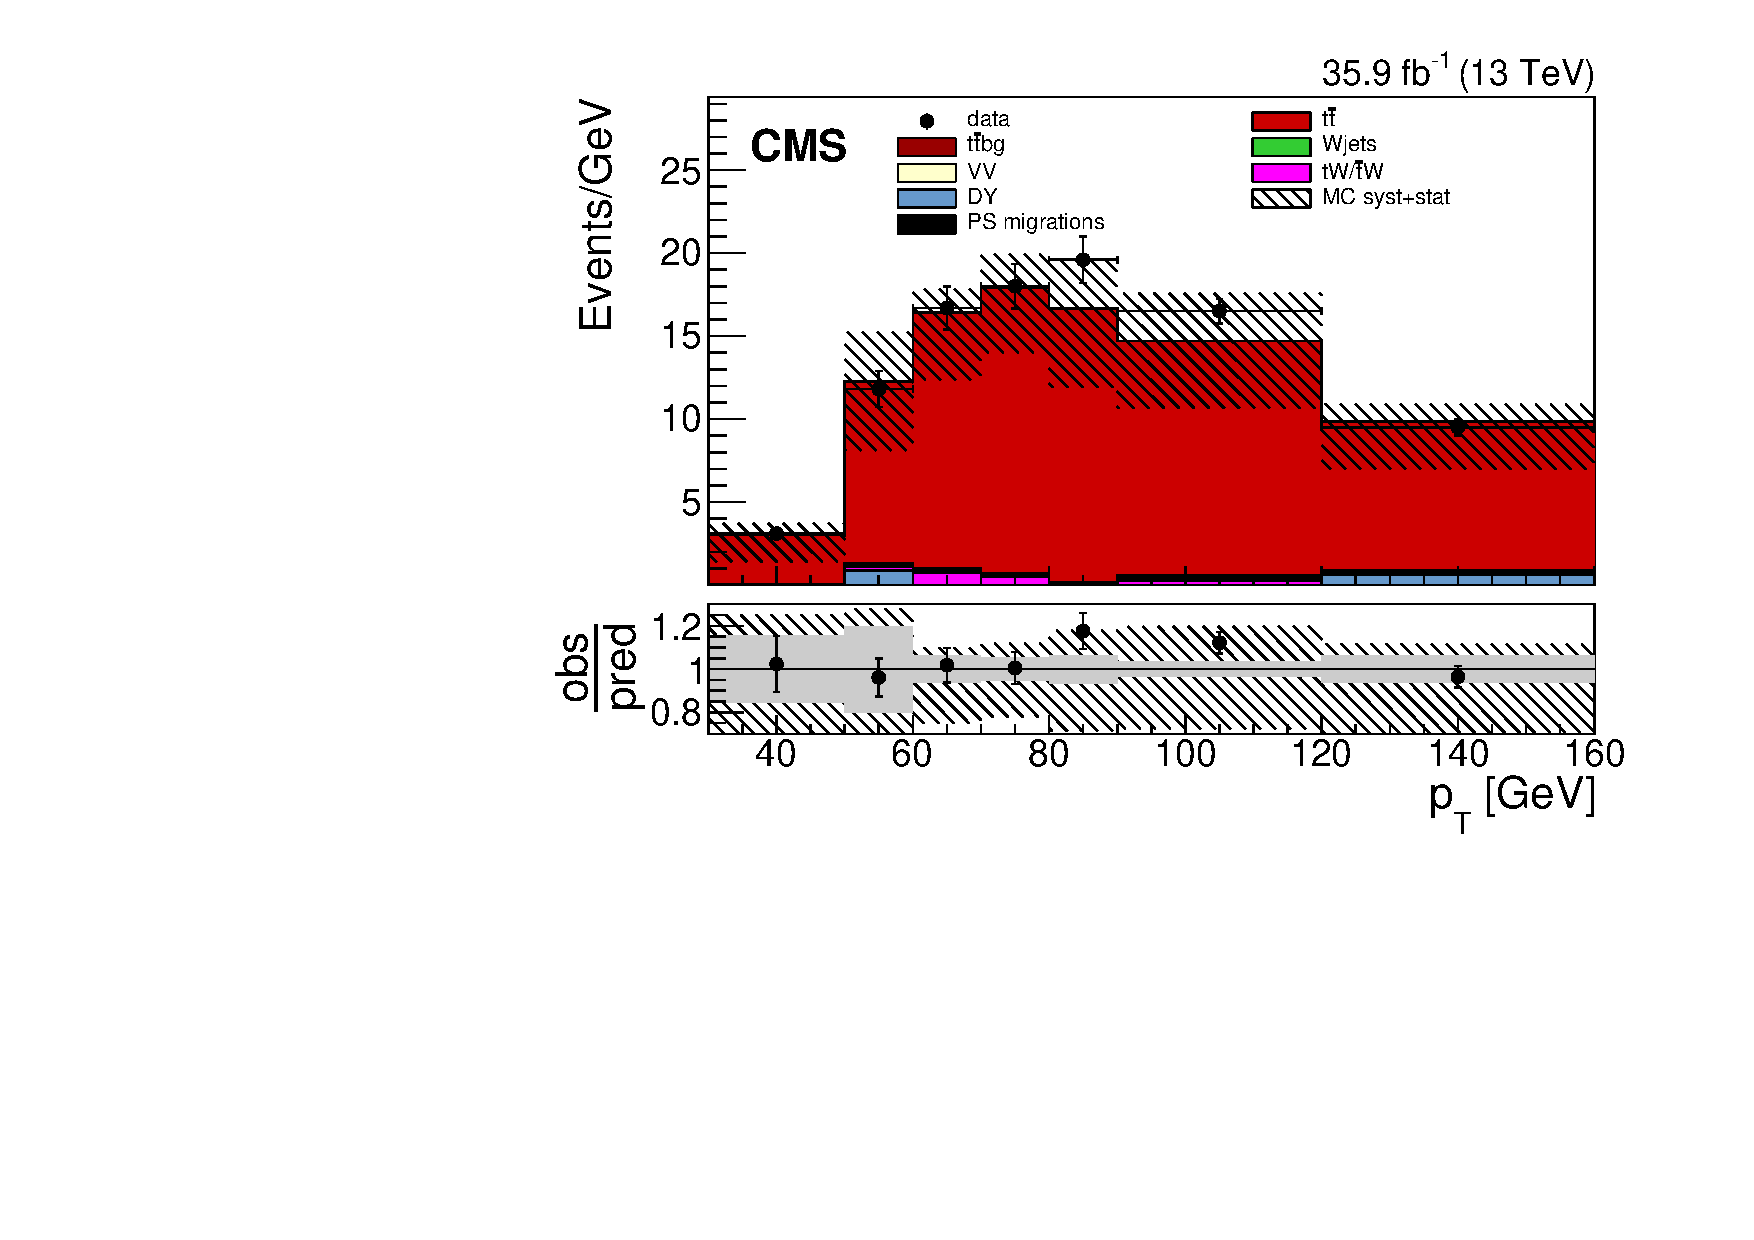
\includegraphics{CrossSection/Figures/ControlPlots/ee_sysnom/lead_jet_pt_2_1_b-jets_step_8.pdf}}\\
        
    \resizebox{0.4 \textwidth}{!}{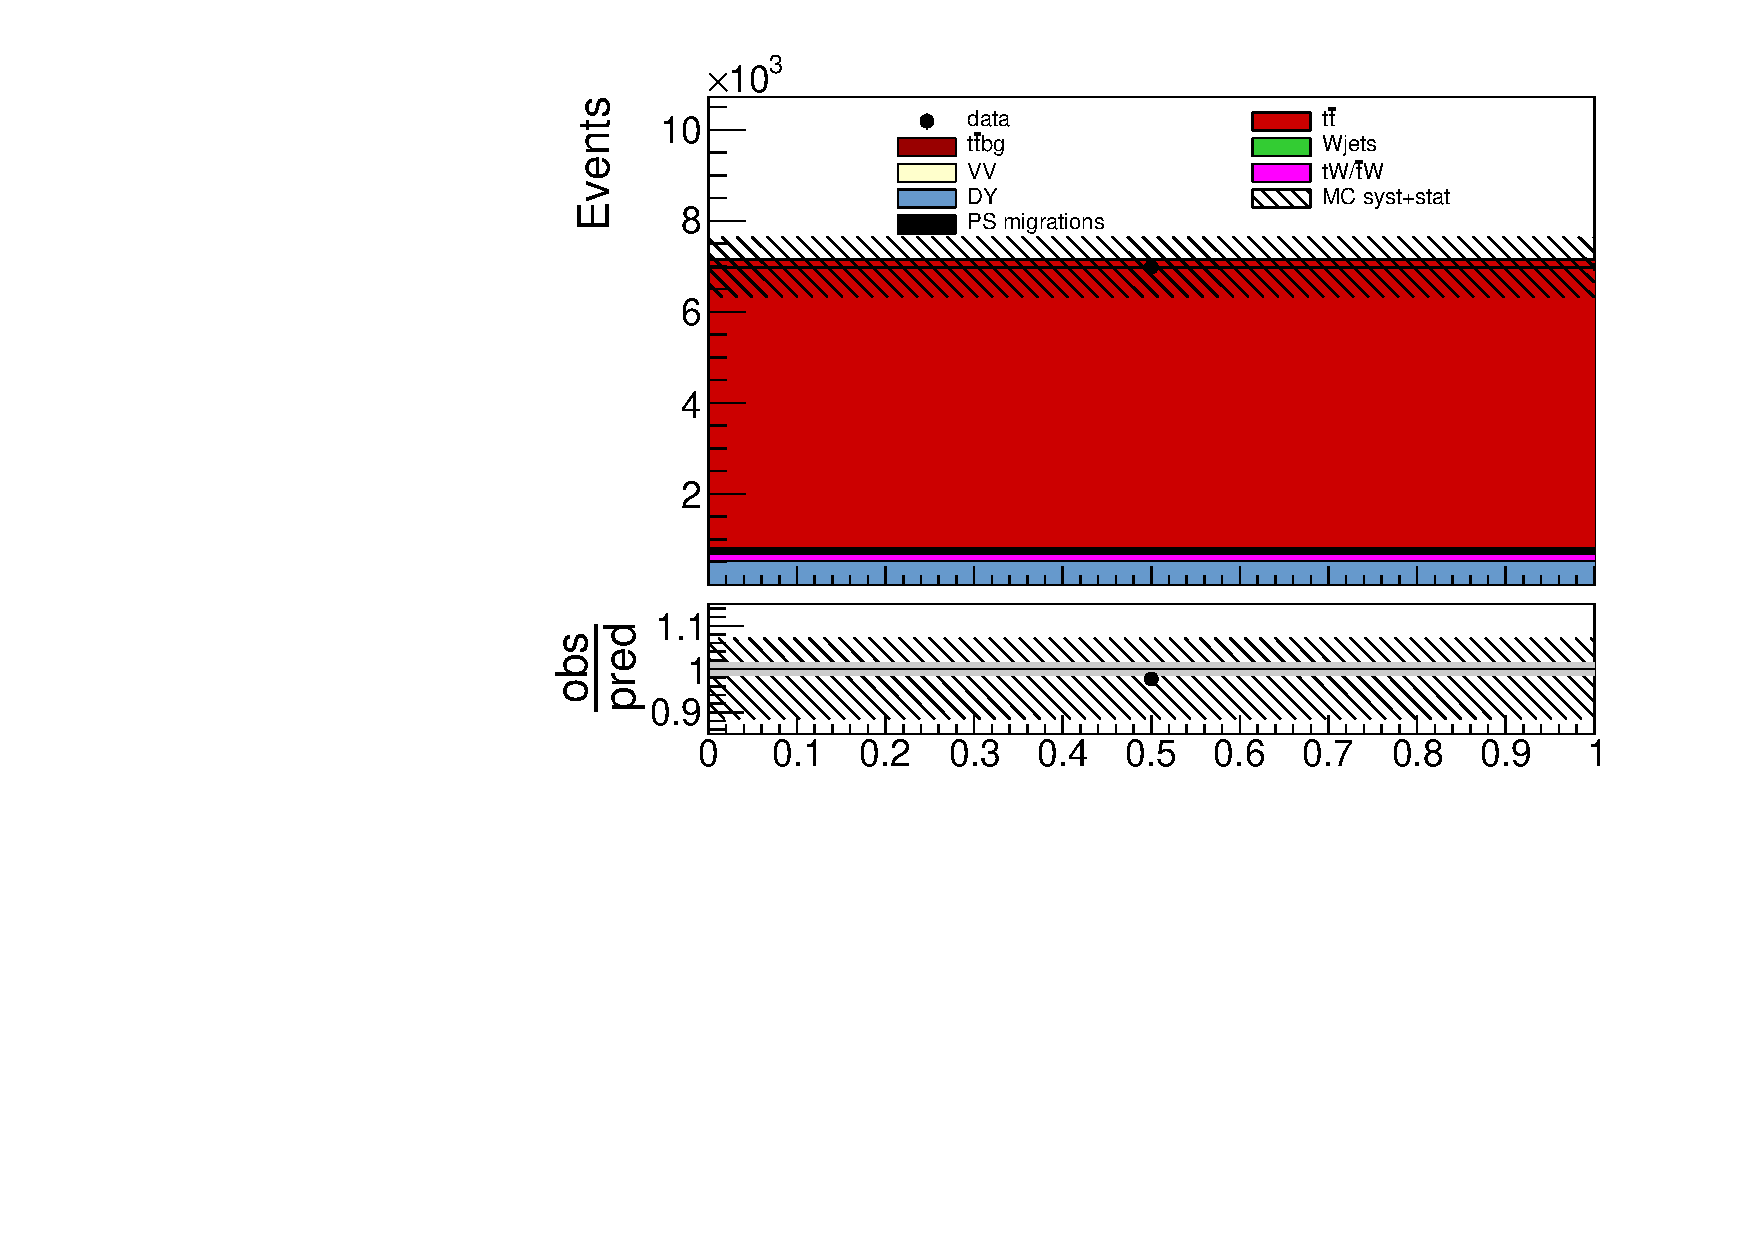
\includegraphics{CrossSection/Figures/ControlPlots/ee_sysnom/total_1_2_b-jets_step_8.pdf}}
    \resizebox{0.4 \textwidth}{!}{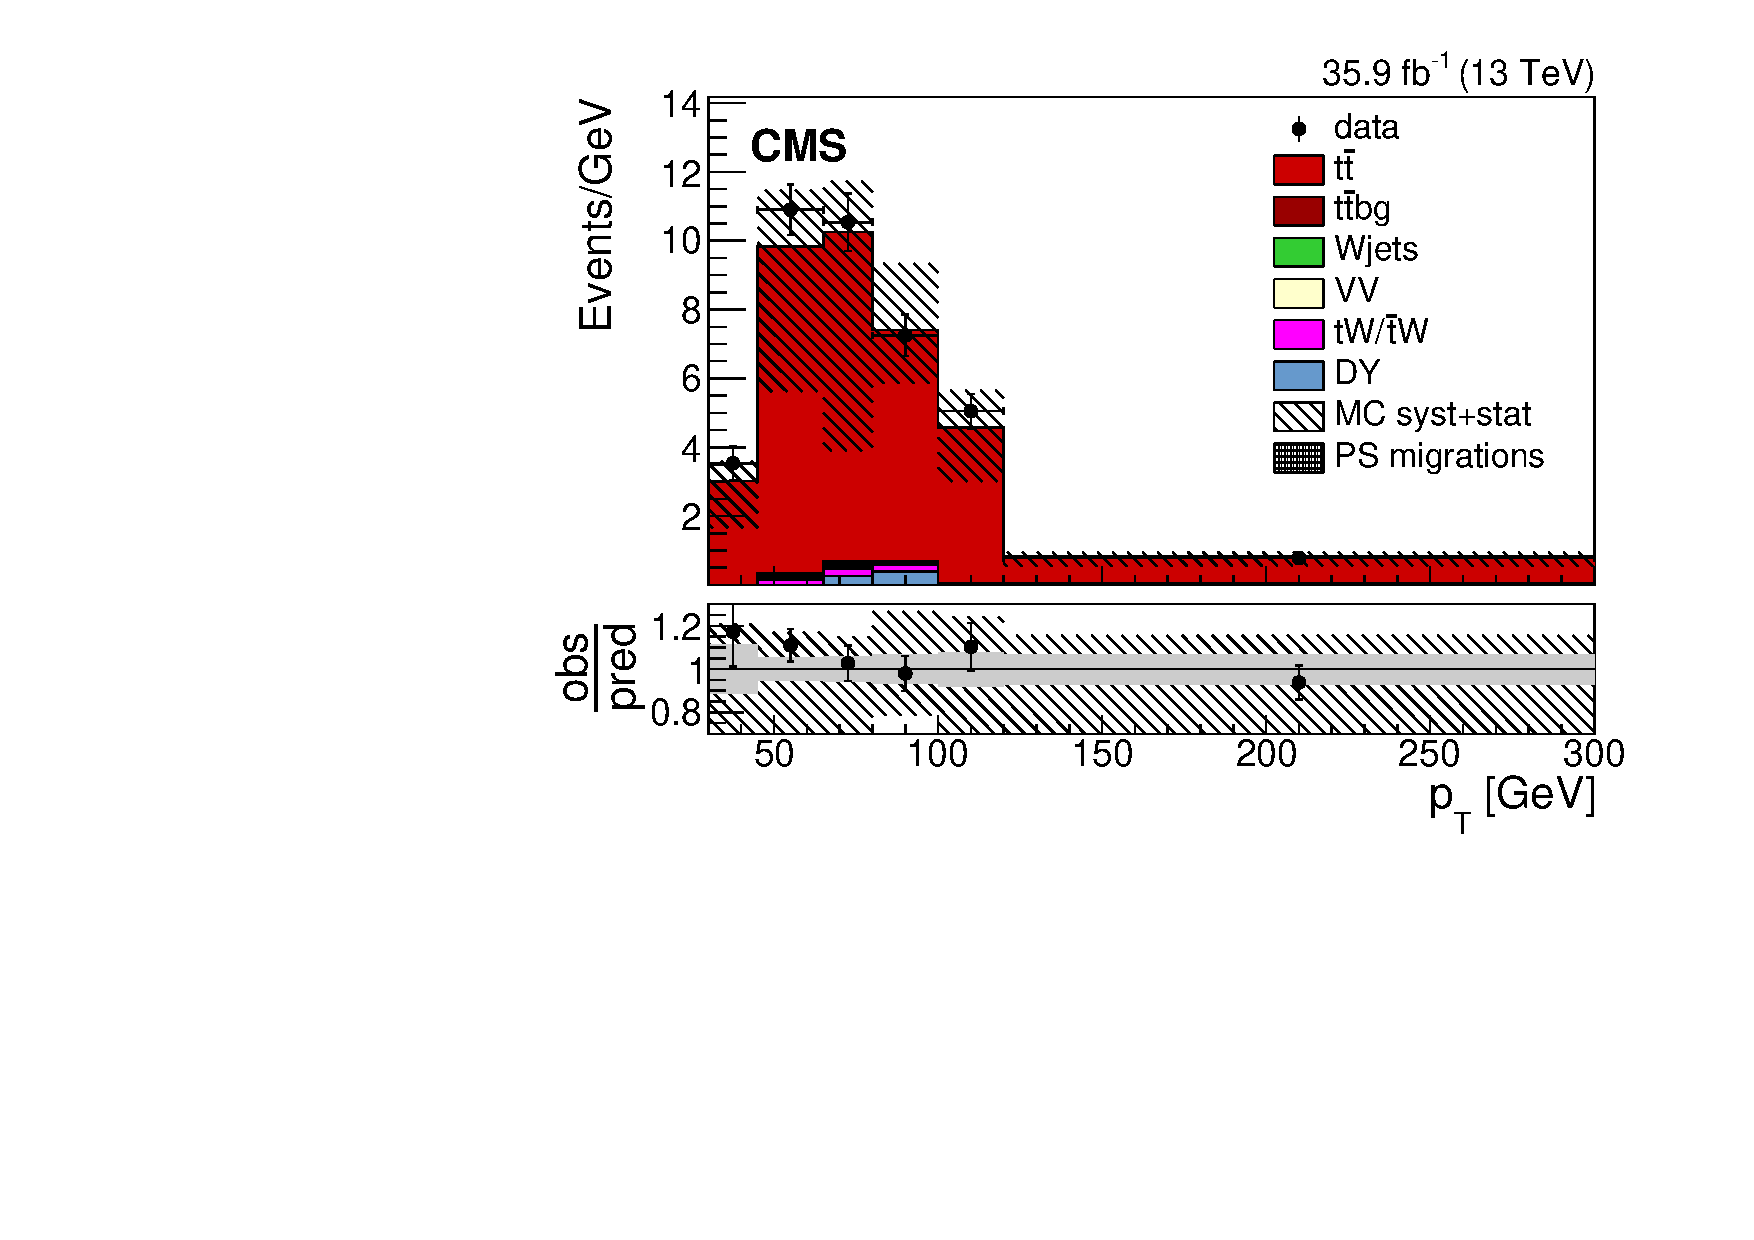
\includegraphics{CrossSection/Figures/ControlPlots/ee_sysnom/second_jet_pt_2_2_b-jets_step_8.pdf}}\\

    \resizebox{0.4 \textwidth}{!}{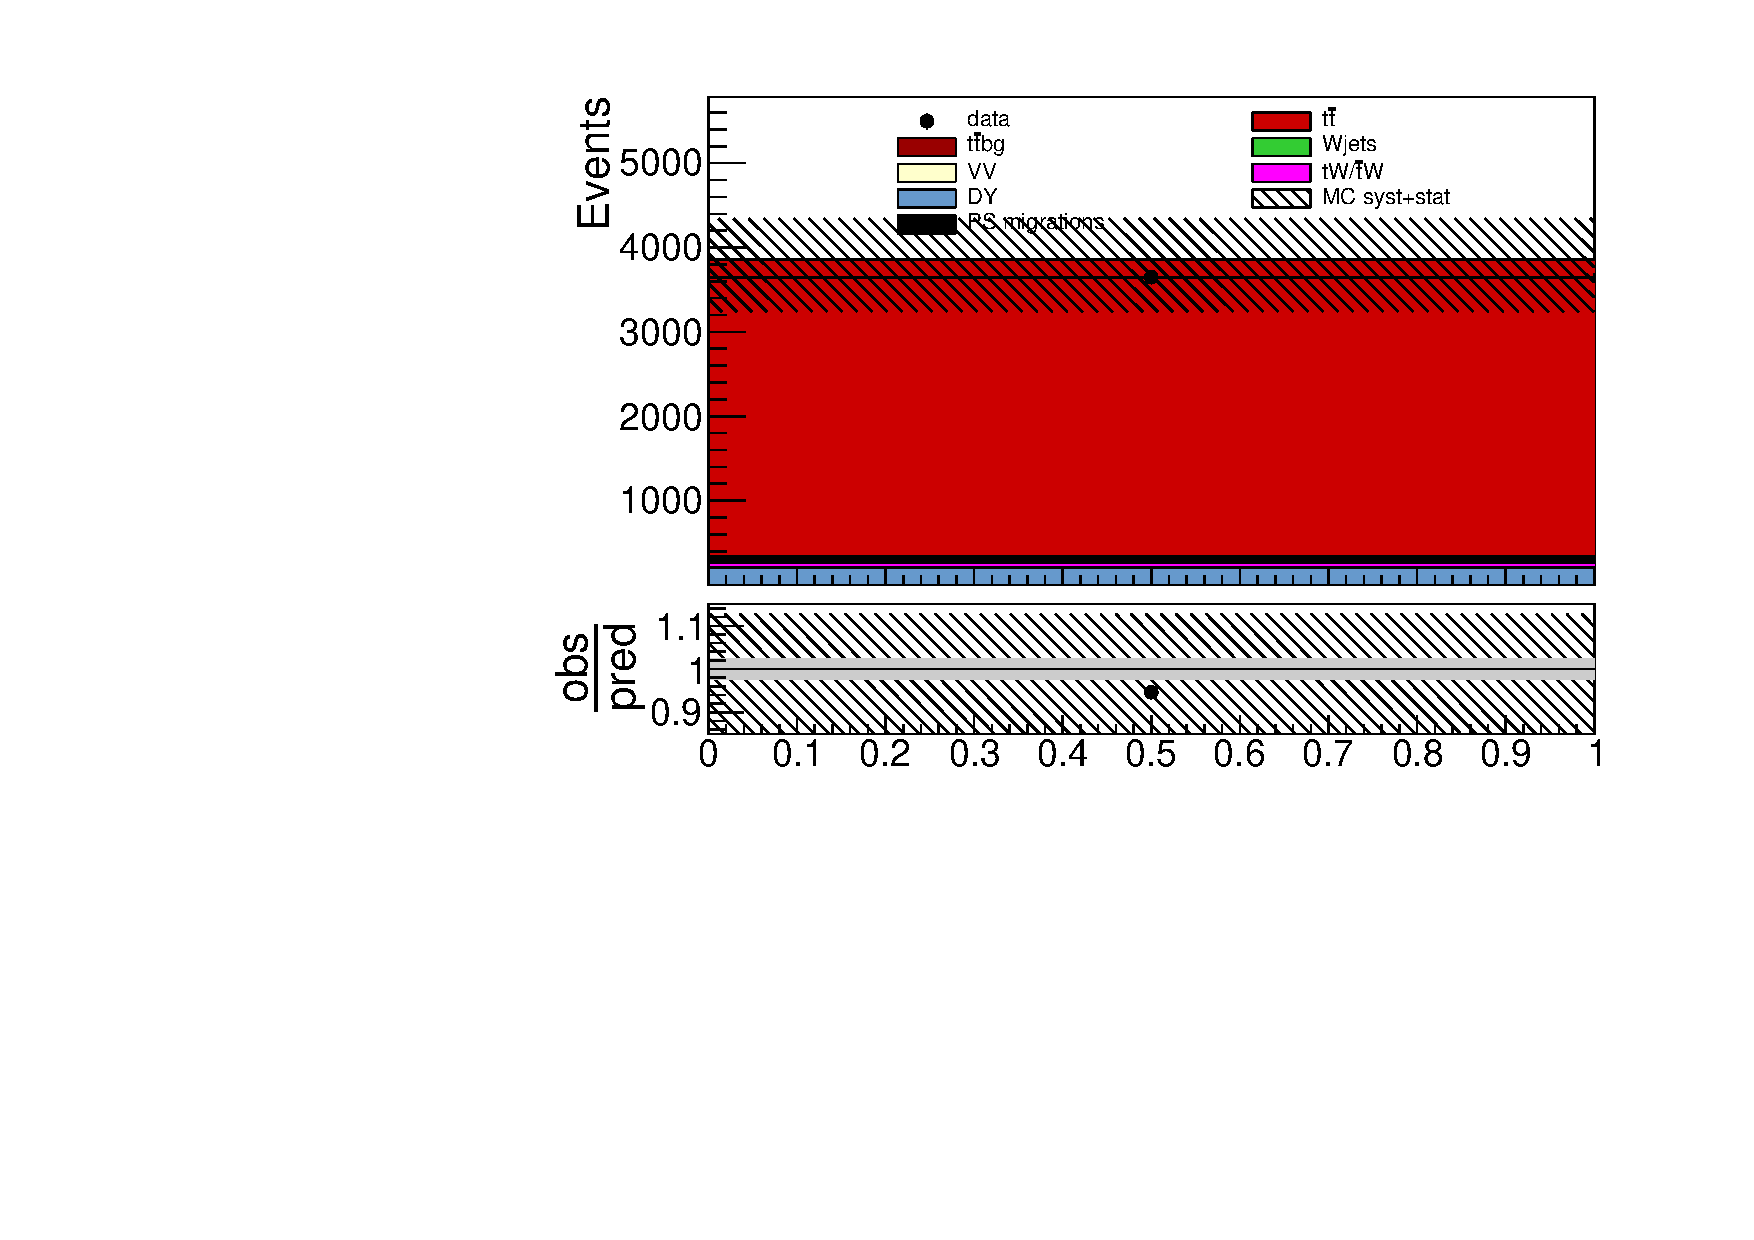
\includegraphics{CrossSection/Figures/ControlPlots/ee_sysnom/total_1_3_b-jets_step_8.pdf}}
    \resizebox{0.4 \textwidth}{!}{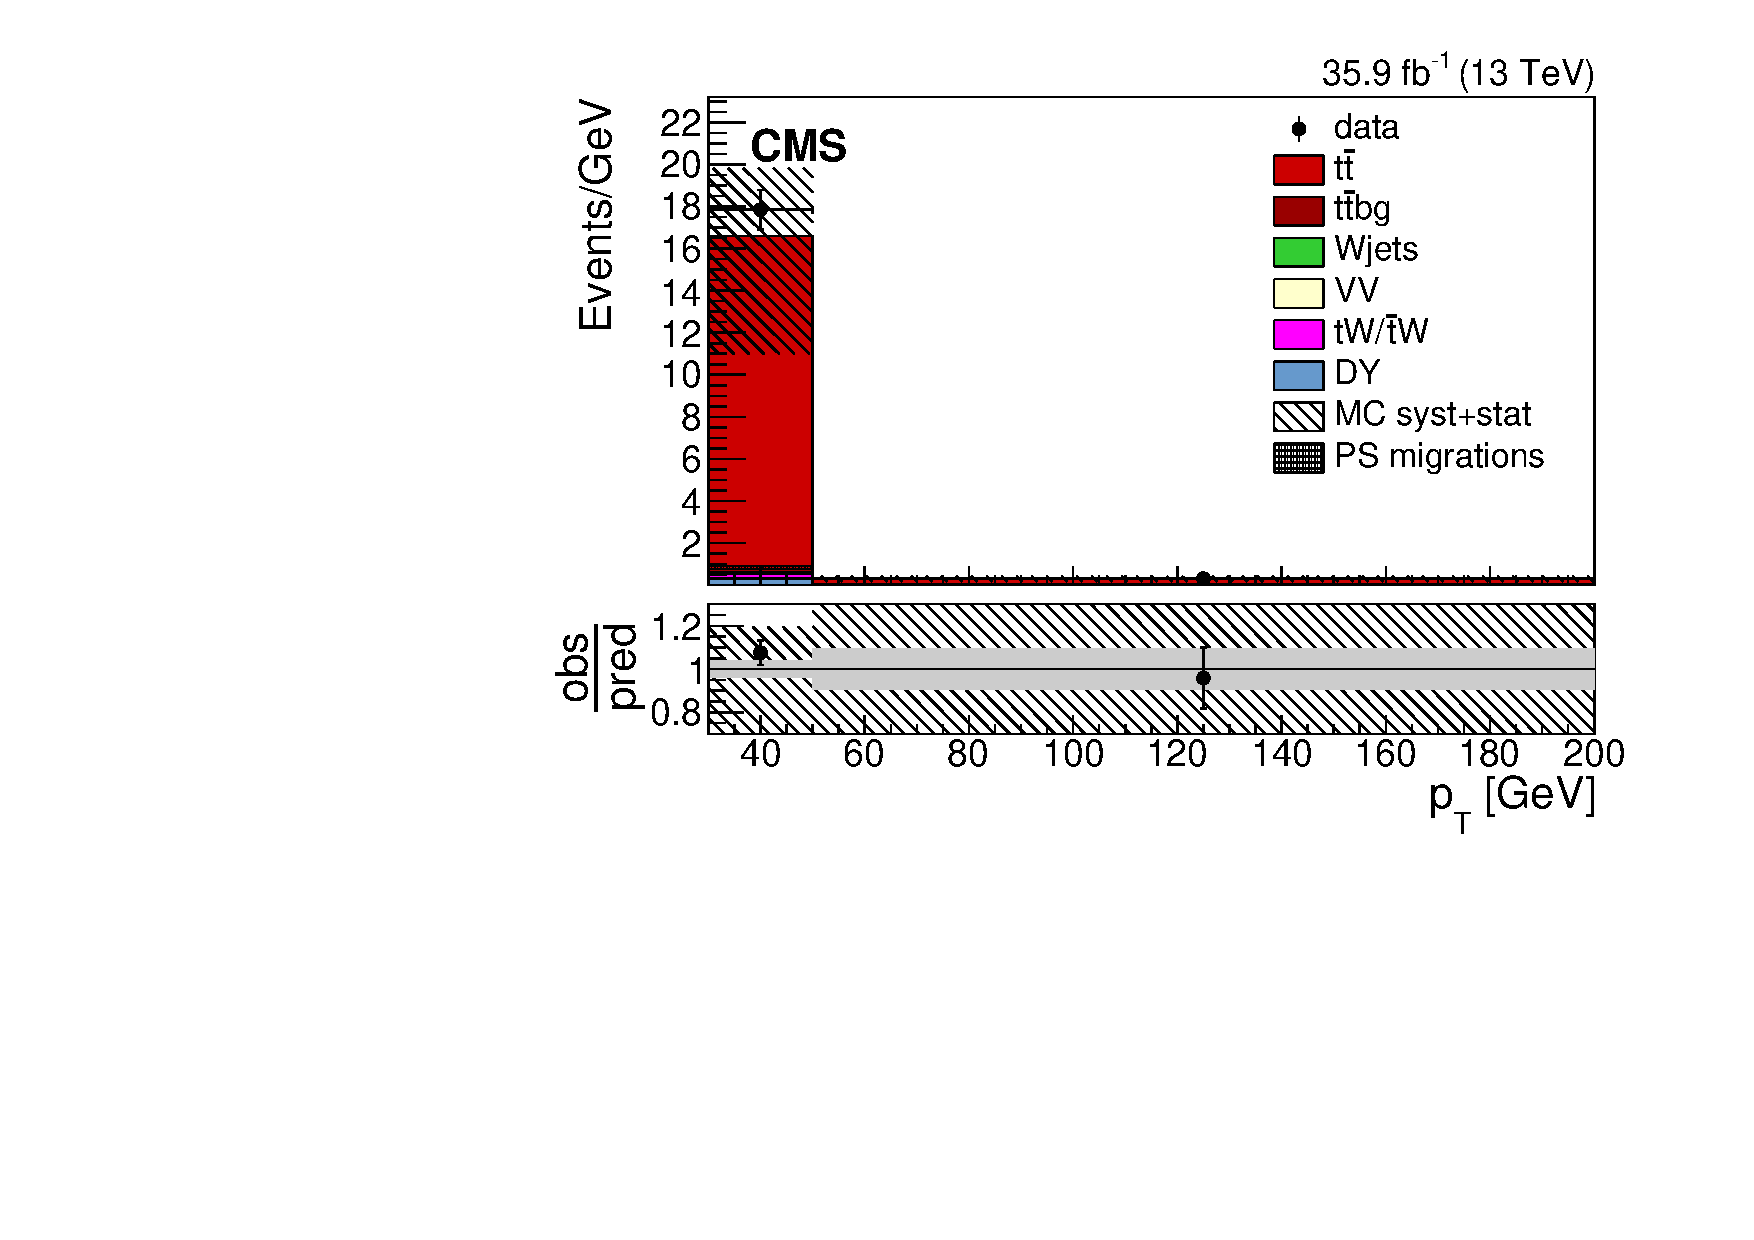
\includegraphics{CrossSection/Figures/ControlPlots/ee_sysnom/third_jet_pt_2_3_b-jets_step_8.pdf}} 
\caption{Pre-Fit distributions (\ee channel): 
  The left column shows events with one b-tagged jet and the total event yield for events with zero (top), one (second from top)
  two (second from bottom) or three or more additional jets (bottom).
  The right column shows events with two b-tagged jets and the total yield for events with zero additional jets (top),
  the trailing jet pt for one (second from top),
  two (second from bottom) or three or more (bottom) additional jets.
  The hatched bands correspond to the total uncertainty on the sum of
  the predicted yields. The ratios of data to the sum of the
  predicted yields are shown at the bottom of each plot. Here, the solid
  gray band represents the contribution of the statistical uncertainty.  
       \label{fig:xsec_ee_inputdistr}}
  \end{center}
\end{figure}


	
\subsection{The Fitting Procedure}
\label{sec:xsec_stat}

Following the description above a binned $\chi^2$ fit is used to extract the cross section and other free parameters.
The basic expression that is minimised can be expressed in the following way:

\begin{equation}
  \chi^2  = \sum_{i} \frac{(n_i-\mu_i)^2}{n_i + \delta_{\mu_i}^2} + \sum_{l} \pi(\omega_l) + \sum_{m} \pi(\lambda_m)
\label{eq:xsec_chisqfunct}
\end{equation}

Here the index $i$ represents a single bin, while $n_i$ is the number of measured events in data, whereas $\mu_i$ is the number
of expected events in simulation. The statistical uncertainty on the expected number of events is introduced in the term $\delta_{\mu_i}$ The terms $\omega_l$ denote the uncertainty on the normalisation of the background contribution and $\lambda_m$
denotes the penalty terms for nuisance parameters with gaussian priors. For these nuisance parameters a unit normal distribution is chosen as penalty term. Nuisance parameters with a uniform prior don't contribute to the penalty terms.
The number of expected events and its uncertainty both depend on the background normalization and all further nuisance parameters.

The events contain a signal as well as a background contribution so $\mu_i$ be written as:

\begin{equation}
\mu_i = s_i(\stt,\vec{\lambda}) 
+ \sum_{l} b_{l,i}(\omega_l,\vec{\lambda}),
\label{eq:xsec_expectev}
\end{equation} 

Here $i$ again denotes the bin, while $l$ denotes the background process. The number of signal events $s_i$ depends on the \ttbar cross section $\stt$ and the nuisance parameters $\vec{\lambda}$.
The number of background events for each background process $b_{l,i}$ also depends on the nuisance parameters and the normalisation of the respective background process $\omega_l$.
In general nuisance parameters related to the detector affect both background and signal, while uncertainties affecting the theory predictions only affect the respective background (see Section \todo{Link to systematics chapter}).

Following the explanation above the number of signal events can be further devided according to the number of b-tagged jets.
Since each of the top quarks decays into a W boson and a b quark it can be assumed that every \ttbar event should contain two jets originating from a b quark.
Any decays of a top quark to a W boson and a light quark can be considered negligible.
It can therefore be assumed that selecting less than two b-tagged jets in a \ttbar event is a measure for the inefficiency of the selection of b-tagged jets.
Following this assumption the number of events in the categories for events with zero or more than two b-tagged jets $s_0$, for events with exactly one $s_1$ and for events with exactly two b-tagged jets $s_2$ can be described as shown in Equation \ref{eq:xsec_nb}. Only events in the \emu channel contribute to category $s_0$.

\begin{eqnarray}
s_0  &=& \mathcal{L}_{\rm int}\stt \epsilon_{ll} \cdot (1-2\epsilon_b(1-C_b\epsilon_b)-C_b\epsilon_b^2) \\
s_1  &=& \mathcal{L}_{\rm int} \stt \epsilon_{ll} \cdot 2 \epsilon_b(1-C_b\epsilon_b) \\
s_2  &=& \mathcal{L}_{\rm int} \stt \epsilon_{ll} \cdot   \epsilon_b^2 C_b 
\label{eq:xsec_nb}.
\end{eqnarray}

Here $\mathcal{L}_{\rm int}$ is the integrated luminosity, $\stt$ is the \ttbar cross section and $\epsilon_ll$ is the efficiency of the dilepton selection.
The b-tag efficiency $\epsilon_b$ includes both the efficiency of the kinematic cuts on the b-jet ($\pt > 30\; \GeV, |\eta|<2.4$) and the efficiency of the b-tagging algorithm.
It is generally assumed that the two b-jets can be identified independently of each other. Any remaining correlation is covered by the parameter $C_b$ that can also be written as
$C_b=4s_{ll}s_2/(s_1+2s_2)^2$ where $\s_{ll}$ is the total number of selected events. 


The number of background events as used in Equation \ref{eq:xsec_expectev} can be decomposed as :

\begin{equation}
b_{l,i} = b_{l,i}^{MC} \cdot (1 + \gamma_l \omega_l),
\label{eq:nbli}
\end{equation}

Here $b_{l,i}^{MC}$ denotes the expected number of events from the simulation of the respective background process and $\gamma_l$ denotes its uncertainty.

The quantities for $\epsilon_{ll}$,$\epsilon_b$, $C_b$, 

Within the fit, the MC simulated quantities $\epsilon_{ll}$, $b_{l,i}$ and $s_{i}$ are taken from simulation and depend on the nuisance parameters $\vec{\lambda}$.
This dependece is modeled with a second order polynomial which is constructed using the nominal and the two systematically varied values of each nuisance parameters $\lambda_m=0,1,-1$.
Some nuisance parameters are based on a one-sided variation so one systematically varied value exists. In these cases the dependence of the simulated quantities is modeled by a linear function.

The MINUIT~\cite{James:1975dr} program is used to minimize the  $\chi^2$ term (see \ref{eq:xsec_chisqfunct} ) as function of the free fit parameters $\stt$, $\vec{\omega}$
and $\vec{\lambda}$. 


\subsection{Extraction from the visual to the Full Phase Space}
\label{sec:xsec_extraction}

